\newpage
\section{ĐỊNH LÍ CÔSIN VÀ ĐỊNH LÍ SIN}
\subsection{LÝ THUYẾT CẦN NHỚ}
\subsubsection{Định lí côsin và định lý sin trong tam giác}
\indam\iconMT{Định lí côsin:}
	\begin{boxdn}
\immini{Cho tam giác $ABC$ với $BC = a$, $CA = b$, $AB = c$. Khi đó
	\begin{align*}
		a^2 &= b^2 + c^2 - 2bc \cos A\\
		b^2 &= a^2 + c^2 - 2ac \cos B \\
		c^2 &= a^2 + b^2 - 2ab \cos C
	\end{align*}}{
	\begin{tikzpicture}[>=stealth,line join=round,line cap=round,font=\footnotesize,scale=1]
		\def\m{1} \def\n{1.6} \def\p{3}
		\path 
		(0,0) coordinate (B)
		(\p,0) coordinate (C)  
		(\m,\n) coordinate (A);
		\foreach \i/\j/\p in {A/B/above, B/C/below left, C/A/below right} {
			\draw(\i) -- (\j);
			\fill(\i) circle (1pt);
			\node[\p] at (\i) {$\i$}; 
		}
		%\path let \p1 = (B), \p2 = (C) in
		%node[below, fill=white, inner sep=1pt] at ($(\p1)!.5!(\p2)$) {$a$};
		\foreach \A/\B/\label/\Nx/\Ny in {B/C/a/0/-0.2,C/A/b/0.2/0.1,A/B/c/-0.1/0.1} {
			\path let \p1 = (\A), \p2 = (\B) in
			node at ($(\p1)!.5!(\p2) + (\Nx,\Ny)$) {$\label$};
		}
		\draw pic[draw,angle radius=2.5mm,angle eccentricity=1.7] {angle = B--A--C}; 
		\draw pic[draw,angle radius=2.5mm,angle eccentricity=1.6,double] {angle = C--B--A};
		\draw pic[fill=gray,angle radius=2.5mm,angle eccentricity=1.6] {angle = A--C--B};
%		\tkzMarkAngle[size=.3*\m](B,A,C)
%		\tkzMarkAngle[size=.4*\m,mark=|](A,C,B)
%		\tkzMarkAngle[size=.3*\m,double](C,B,A)
	\end{tikzpicture}
}	
	\end{boxdn}

\indam\iconMT{Định lí sin:}
\begin{boxdn}
\immini{Cho tam giác $ABC$ với $BC = a$, $CA = b$, $AB = c$. Khi đó
	\[\dfrac{a}{\sin A} = \dfrac{b}{\sin B} = \dfrac{c}{\sin C} = 2R
	\]
	trong đó $R$ là bán kính đường tròn ngoại tiếp tam giác $ABC$.}{
	\begin{tikzpicture}[>=stealth,line join=round,line cap=round,font=\footnotesize,scale=0.8]
		\def\m{1} \def\n{2} \def\p{3}
		\path 
		(0,0) coordinate (B) 
		(\p,0) coordinate (C)  
		(\m+1,\n) coordinate (A);
		\begin{scope}[scale=1.25]
			\path 
			(barycentric cs:A=1,B=1) coordinate (ab) 
			(barycentric cs:A=1,C=1) coordinate (ac) 
			([rotate around={90:(ab)}]B) coordinate (abt) 
			([rotate around={90:(ac)}]C) coordinate (act) 
			(intersection of ab--abt and ac--act) coordinate (I);
			\draw (I) let \p1=($(I)-(A)$),\n1={veclen(\x1,\y1)} in circle (\n1);
			\fill (I) circle (1pt) node[shift={(-45:5pt)}] {$I$};
			%\draw[thick,blue]  let \p1=($(A)-(I)$), \n1={veclen(\x1,\y1)}
			%in pic[draw,angle radius=\n1]{angle = C--I--A}
			%;
		\end{scope}	
		\foreach \i/\j/\p in {A/B/above, B/C/below left, C/A/below right} {
			\draw(\i) -- (\j);
			\fill(\i) circle (1pt);
			\node[\p] at (\i) {$\i$}; 
		}
		\foreach \A/\B/\label/\Nx/\Ny in {B/C/a/0/-0.2,C/A/b/0.2/0.1,A/B/c/-0.1/0.1} {
			\path let \p1 = (\A), \p2 = (\B) in
			node at ($(\p1)!.5!(\p2) + (\Nx,\Ny)$) {$\label$};
		}
		\draw pic[draw,angle radius=2.5mm,angle eccentricity=1.7] {angle = B--A--C}; 
		\draw pic[draw,angle radius=2.5mm,angle eccentricity=1.6,double] {angle = C--B--A};
		\draw pic[fill=gray,angle radius=2.5mm,angle eccentricity=1.6] {angle = A--C--B};
%		\tkzMarkAngle[size=.3*\m](B,A,C)
%		\tkzMarkAngle[size=.4*\m,mark=|](A,C,B)
%		\tkzMarkAngle[size=.3*\m,double](C,B,A)	
		\draw (I)--(A) node [midway, shift={(-45:5pt)}] {$R$};
	\end{tikzpicture}
}	
\end{boxdn}
\begin{khung4}{Hệ quả}
\begin{itemize}
\item Tính góc theo độ dài $3$ cạnh
\[\cos A = \dfrac{b^2 + c^2 - a^2}{2bc}, \qquad\cos B = \dfrac{c^2 + a^2 - b^2}{2ca}, \qquad\cos C = \dfrac{a^2 + b^2 - c^2}{2ab}.
\]
\item Tính cạnh theo bán kính đường tròn ngoại tiếp tam giác và số đo góc đối diện 
\[a = 2R \sin A, 	\qquad b = 2R \sin B, \qquad c = 2R \sin C.
\]
\item Tính bán kính đường tròn ngoại tiếp tam giác theo cạnh và số đo góc đối diện
\[a = 2R \sin A, \qquad b = 2R \sin B, \qquad	c = 2R \sin C.
\]
\end{itemize}
\end{khung4}
\subsubsection{Các công thức diện tích tam giác}
%\indam{}
\begin{boxdn}
	\immini{Cho tam giác $ABC$ với $BC = a$, $CA = b$, $AB = c$. Ký hiệu $S$ là diện tích và $p=\dfrac{a+b+c}{2}$ là nửa chu vi của tam giác $ABC$. Khi đó
		\begin{itemize}
			%	\item $S = \dfrac{1}{2}ah_a = \dfrac{1}{2}bh_b = \dfrac{1}{2}ch_c$
			\item $S = \dfrac{1}{2}ab\sin C = \dfrac{1}{2}bc\sin A = \dfrac{1}{2}ac\sin B$
			\item $S = \sqrt{p(p - a)(p - b)(p - c)}$ \quad (công thức \textbf{Heron}).
			\item $S = \dfrac{abc}{4R}$  \quad ($R$ là bán kính đường tròn ngoại tiếp tam giác $ABC$).
			\item $S = pr$  \quad ($r$ là bán kính đường tròn nội tiếp tam giác $ABC$).
		\end{itemize}
	}{
		\begin{tikzpicture}[>=stealth,line join=round,line cap=round,font=\footnotesize,scale=1]
			\def\m{1} \def\n{2} \def\p{3}
			\path 
			(0,0) coordinate (B) 
			(\p,0) coordinate (C)  
			(\m,\n) coordinate (A);
			\coordinate (H) at ($(B)!(A)!(C)$);
			\foreach \i/\j/\p in {A/B/above, B/C/below left, C/A/below right} {
				\draw(\i) -- (\j);
				\fill(\i) circle (1pt);
				\node[\p] at (\i) {$\i$}; 
			}
			\foreach \A/\B/\label/\Nx/\Ny in {B/C/a/0/-0.2,C/A/b/0.2/0.1,A/B/c/-0.1/0.1} {
				\path let \p1 = (\A), \p2 = (\B) in
				node at ($(\p1)!.5!(\p2) + (\Nx,\Ny)$) {$\label$};
			}
		\draw pic[draw,angle radius=2.5mm,angle eccentricity=1.7] {angle = A--C--B}; 
%			\tkzMarkAngle[size=.3*\m](A,C,B)
			\path let \p1 = (A), \p2 = (H) in
			node[right] at ($(\p1)!.5!(\p2)$) {$h_a$};
			\draw(A) -- (H);
			\pic[draw,angle radius=5*\m]{right angle = A--H--C};
		\end{tikzpicture}
		\\[0.3cm]
		$\boxed{S = \dfrac{1}{2}ah_a}$
	}	
\end{boxdn}
\begin{khung4}{Chú ý}
\ding{118} Định lý sin và định lý côsin là \textbf{Hai viên ngọc quý} của hình học phẳng trong vấn đề giải tam giác nói riêng, trong các vấn đề về đo đạc nói chung.
\end{khung4}

%-------------------------------------------------------------------------------------------------------------
\subsection{PHÂN LOẠI VÀ PHƯƠNG PHÁP GIẢI TOÁN}
\begin{dang}{Áp dụng định lý côsin và hệ quả}	
\noindent
\begin{minipage}[c]{0.33\textwidth}
\vspace{-0.5em}
	\qquad \textbf{Công thức}
	\begin{itemize}	
\vspace{1em}
		\item[\ding{172}] $a^2 = b^2 + c^2 - 2bc \cos A$
\vspace{1em}
		\item[\ding{173}] $b^2 = c^2 + a^2 - 2ca \cos B$
\vspace{1em}
		\item[\ding{174}] $c^2 = a^2 + b^2 - 2ab \cos C$		
	\end{itemize}
\end{minipage}
\hfill
\begin{minipage}[c]{0.33\textwidth}
	\qquad \textbf{Hệ quả}
\begin{itemize}
	\item[\tiny\ding{117}] $\cos A = \dfrac{b^2 + c^2 - a^2}{2bc}$
	\item[\tiny\ding{117}] $\cos B = \dfrac{c^2 + c^2 - b^2}{2ca}$
	\item[\tiny\ding{117}] $\cos C = \dfrac{a^2 + b^2 - c^2}{2ab}$
	\end{itemize}
\end{minipage}
\hfill
\begin{minipage}[c]{0.32\textwidth}
	\begin{center}
		\begin{tikzpicture}[>=stealth,line join=round,line cap=round,font=\footnotesize,scale=1]
	\def\m{1} \def\n{1.4} \def\p{3}
	\path 
	(0,0) coordinate (B)
	(\p,0) coordinate (C)  
	(\m,\n) coordinate (A);
	\foreach \i/\j/\p in {A/B/above, B/C/below left, C/A/below right} {
		\draw(\i) -- (\j);
		\fill(\i) circle (1pt);
		\node[\p] at (\i) {$\i$}; 
	}
	%\path let \p1 = (B), \p2 = (C) in
	%node[below, fill=white, inner sep=1pt] at ($(\p1)!.5!(\p2)$) {$a$};
	\foreach \A/\B/\label/\Nx/\Ny in {B/C/a/0/-0.2,C/A/b/0.2/0.1,A/B/c/-0.1/0.1} {
		\path let \p1 = (\A), \p2 = (\B) in
		node at ($(\p1)!.5!(\p2) + (\Nx,\Ny)$) {$\label$};
	}
	\draw pic[draw,angle radius=2.5mm,angle eccentricity=1.7] {angle = B--A--C}; 
	\end{tikzpicture}
	\end{center}
	\[\boxed{\widehat A+\widehat B+\widehat C=180^\circ}
	\]
\end{minipage}
\end{dang}

%Bai1
\begin{vd}%[0H4H2-1]
Cho $ABC$ biết $b=AC = 8$, $a=BC = 12$ và $\widehat{C} = 120^\circ$. Tính cạnh $c$ và $\cos A$. 
\loigiai{
\immini{
Theo định lí côsin, ta có:
\[
c^2 = a^2 + b^2 - 2 a b \cos \widehat{C}
= 12^2 + 8^2 - 2 \cdot 12 \cdot 8 \cdot \cos 120^\circ
= 304\Rightarrow c = 4\sqrt{19}.\]
Theo định lí côsin, ta có:
\[
\cos A = \dfrac{c^2 + b^2 - a^2}{2 c b}
= \dfrac{\left(4\sqrt{19}\right)^2 + 8^2 - 12^2}{2 \cdot 4\sqrt{19} \cdot 8}=\dfrac{7\sqrt{19}}{38}.
\]
Vậy $c =4\sqrt{19}$, $\cos A=\dfrac{7\sqrt{19}}{38}$.}{
\begin{tikzpicture}[>=stealth,line join=round,line cap=round,font=\footnotesize,scale=1]
\def\m{4.6} \def\n{2} \def\p{3.5}
\path
(0,0) coordinate (B)
(\p,0) coordinate (C)
(\m,\n) coordinate (A);
\foreach \i/\j/\p in {A/B/above, B/C/below, C/A/below} {
\draw(\i) -- (\j);
\fill(\i) circle (1pt);
\node[\p] at (\i) {$\i$};
}
%\path let \p1 = (B), \p2 = (C) in
%node[below, fill=white, inner sep=1pt] at ($(\p1)!.5!(\p2)$) {$a$};
\foreach \A/\B/\label/\Nx/\Ny in {C/A/8/0.2/0,C/B/12/-0.1/-0.2} {
\path let \p1 = (\A), \p2 = (\B) in
node at ($(\p1)!.5!(\p2) + (\Nx,\Ny)$) {$\label$};
}
	\draw pic[draw,angle radius=2.5mm,angle eccentricity=1.7,"$120^\circ$"] {angle = A--C--B}; 
%\tkzMarkAngle[size=.3](A,C,B)
%\tkzLabelAngle[pos=.5](A,C,B){\footnotesize $115^\circ$}
\end{tikzpicture}
}
}
\end{vd}
%Bai2
\vspace{0.5em} 
\begin{vd}%[0H4H2-1]
	Cho tam giác $ABC$ có $a=7$, $b=8$, $c=9$. Tính các góc của tam giác (làm tròn kết quả đến hàng phần mười theo đơn vị độ).
\loigiai{
Theo định lí côsin, ta có:
	\[
	\cos A = \dfrac{b^2 + c^2 - a^2}{2bc} = \dfrac{64 + 81 - 49}{2\cdot 8 \cdot 9} = \dfrac{96}{144} = \dfrac{2}{3}\Rightarrow \widehat A \approx 48{,}2^\circ.
	\]
	\[
	\cos B = \dfrac{a^2 + c^2 - b^2}{2ac} = \dfrac{49 + 81 - 64}{2\cdot 7 \cdot 9} = \dfrac{66}{126} = \dfrac{11}{21} \Rightarrow \widehat B \approx 58{,}4^\circ.
	\]
	Theo định lý về tổng ba góc trong tam giác, suy ra $C = 180^\circ - \widehat A - \widehat B \approx 73{,}4^\circ$.\\
	Vậy $\widehat A \approx 48{,}2^\circ$, $\widehat B \approx 58{,}4^\circ$, $C\approx 73{,}4^\circ$.
	} 	
\end{vd}
%Bai3
\vspace{0.5em} 
\begin{vd}%[0H4H2-1]
	Cho tam giác $ABC$.
	\begin{itemize}
	 \item [1)] Biết rằng $b^2 + c^2 = a^2+bc$. Tính số đo góc $A$.
	 \item [2)] Biết rằng $c =2b\cos A$. Chứng tỏ tam giác $ABC$ cân.
	\end{itemize}	
	\loigiai{
	\begin{itemize}
		\item [1)] Theo định lí côsin, ta có $a^2 = b^2 + c^2 - 2bc \cos A$.\\
		Mặt khác, theo giả thiết $b^2 + c^2 = a^2+bc$ nên
		\[a^2 = a^2+bc - 2bc \cos A\Rightarrow bc = 2bc \cos A\Rightarrow \cos A=\dfrac{1}{2}\Rightarrow \widehat A= 60^\circ.
		\]
	Vậy $\widehat A= 60^\circ$.
		\item [2)] Ta có 
		\[c=2b\cos A\Rightarrow c=2b\cdot\dfrac{b^2+c^2-a^2}{2bc}\Rightarrow c^2=b^2+c^2-a^2\Rightarrow b^2-a^2=0\Rightarrow a=b.
		\]
	\end{itemize}	
	Vậy tam giác $ABC$ cân tại $C$.
	} 	
\end{vd}

%%-------------------%
\begin{dang}{Áp dụng định lý sin và hệ quả}	
	\noindent
	\begin{minipage}[c]{0.65\textwidth}
		\qquad \textbf{Công thức}
		\[\dfrac{a}{\sin A} = \dfrac{b}{\sin B}=\dfrac{c}{\sin C} =2R,
		\]
\begin{center}
trong đó $R$ là bán kính đường tròn ngoại tiếp tam giác $ABC$.
\end{center}
		\qquad \textbf{Hệ quả}
		\begin{itemize}
			\item[\tiny\ding{117}] $a = \dfrac{b\sin A}{\sin B}=\dfrac{c\sin A}{\sin C}$.	
			\item[\tiny\ding{117}] $\sin A=\dfrac{a}{2R}$;\quad $\sin B=\dfrac{b}{2R}$;\quad $\sin C=\dfrac{c}{2R}$.
			\item[\tiny\ding{117}] $a=2R\sin A$;\quad $b=2R\sin B$;\quad $c=2R\sin C$.
		\end{itemize}
	\end{minipage}		
	\begin{minipage}[c]{0.3\textwidth}
		\begin{center}
	\begin{tikzpicture}[>=stealth,line join=round,line cap=round,font=\footnotesize,scale=0.8]
			\def\m{0.5} \def\n{2.5} \def\p{4.5}
			\path 
			(0,0) coordinate (B) 
			(\p,0) coordinate (C)  
			(\m+1,\n) coordinate (A);
			\begin{scope}[scale=1.25]
					\path 
					(barycentric cs:A=1,B=1) coordinate (ab) 
					(barycentric cs:A=1,C=1) coordinate (ac) 
					([rotate around={90:(ab)}]B) coordinate (abt) 
					([rotate around={90:(ac)}]C) coordinate (act) 
					(intersection of ab--abt and ac--act) coordinate (I);
					\draw (I) let \p1=($(I)-(A)$),\n1={veclen(\x1,\y1)} in circle (\n1);
					\fill (I) circle (1pt) node[shift={(-45:5pt)}] {$I$};
					%\draw[thick,blue]  let \p1=($(A)-(I)$), \n1={veclen(\x1,\y1)}
					%in pic[draw,angle radius=\n1]{angle = C--I--A}
					%;
				\end{scope}	
			\foreach \i/\j/\p in {A/B/above, B/C/below left, C/A/below right} {
					\draw(\i) -- (\j);
					\fill(\i) circle (1pt);
					\node[\p] at (\i) {$\i$}; 
				}
			\foreach \A/\B/\label/\Nx/\Ny in {B/C/a/0/-0.2,C/A/b/0.2/0.1,A/B/c/-0.1/0.1} {
					\path let \p1 = (\A), \p2 = (\B) in
					node at ($(\p1)!.5!(\p2) + (\Nx,\Ny)$) {$\label$};
				}
			\draw pic[draw,angle radius=2.5mm,angle eccentricity=1.7] {angle = B--A--C}; 
			\draw pic[draw,angle radius=2.5mm,angle eccentricity=1.6,double] {angle = C--B--A};
			\draw pic[fill=gray,angle radius=2.5mm,angle eccentricity=1.6] {angle = A--C--B};
	%		\tkzMarkAngle[size=.3*\m](B,A,C)
	%		\tkzMarkAngle[size=.4*\m,mark=|](A,C,B)
	%		\tkzMarkAngle[size=.3*\m,double](C,B,A)	
			\draw (I)--(A) node [midway, shift={(-30:5pt)}] {$R$};
		\end{tikzpicture}
		\end{center}
		\[\boxed{\widehat A>\widehat B>\widehat C\Leftrightarrow a>b>c}	
		\]
	\end{minipage}
\end{dang}

%Bai4
\begin{vd}%[0H4H2-1]
Cho tam giác $ABC$ có $\widehat{A} = 72^\circ$, $\widehat{B} = 83^\circ$, $BC = 18$. Tính độ dài các cạnh $AB$, $CA$ của $ABC$ \textit{(làm tròn kết quả đến hàng phần mười)}.
\loigiai{
\immini{
Đặt $a = BC$, $b = AC$, $c = AB$. \\
Ta có $a = 18$, $\widehat{C} = 180^\circ - (72^\circ + 83^\circ) = 25^\circ$.\\
Từ định lý sin, ta có
\begin{align*}
&AC = b = \dfrac{a \sin B}{\sin A} = \dfrac{18 \cdot \sin 83^\circ}{\sin 72^\circ} \approx 18{,}8; \\
&AB = c = \dfrac{a \sin C}{\sin A} = \dfrac{18 \cdot \sin 25^\circ}{\sin 72^\circ} \approx 8{,}0.
\end{align*}}{
\begin{tikzpicture}[>=stealth,line join=round,line cap=round,font=\footnotesize,scale=1]
\def\m{0.3} \def\n{2.2} \def\p{5}
\path
(0,0) coordinate (B)
(\p,0) coordinate (C)
(\m,\n) coordinate (A);
\foreach \i/\j/\p in {A/B/above, B/C/below, C/A/below} {
\draw(\i) -- (\j);
\fill(\i) circle (1pt);
\node[\p] at (\i) {$\i$};
}
\node at ($(B)!.5!(C) + (0,-.2)$) {$18$};
	\draw pic[draw,angle radius=2.5mm,angle eccentricity=1.7,"$72^\circ$"] {angle = B--A--C}; 
	\draw pic[draw,angle radius=2.5mm,angle eccentricity=2,double,"$83^\circ$"] {angle = C--B--A};
\end{tikzpicture}
}
}
\end{vd}

%Bai5
\vspace{0.5em} 
\begin{vd}%[0H4H2-1]
	Cho tam giác $ABC$ có $a=R$. Tính số đo góc $A$.
	\loigiai{
		Theo định lí sin, ta có $\sin A=\dfrac{a}{2R}$\\
		Mặt khác, theo giả thiết $a= R$ nên
		\[\sin A=\dfrac{R}{2R}=\dfrac{1}{2}\Rightarrow  \hoac{&\widehat A= 30^\circ\\&\widehat A= 150^\circ.}
		\]
	} 	
\end{vd}

%Bai6
\vspace{0.5em} 
\begin{vd}%[0H4H2-1]
	Chứng tỏ rằng, trong tam giác $ABC$ ta luôn có
	\[\cot A+\cot B+\cot C=\dfrac{\left(a^2+b^2+c^2\right)R}{abc}.
	\]
	\loigiai{
	Theo định lí côsin, ta có:
		\[
		\cos A = \dfrac{b^2 + c^2 - a^2}{2bc} \Rightarrow \dfrac{\cos A}{a}=\dfrac{b^2 + c^2 - a^2}{2abc}
		\]
		Tương tự như thế ta có
		\[
		\dfrac{\cos A}{a}+\dfrac{\cos B}{b}+\dfrac{\cos C}{c}=\dfrac{b^2 + c^2 - a^2}{2abc}+\dfrac{c^2 + a^2 - b^2}{2abc}+\dfrac{a^2 + b^2 - c^2}{2abc}=\dfrac{a^2 + b^2 + c^2}{2abc}.\quad (1)
		\]
	Theo định lí sin, ta có: $a=2R\sin A$; $b=2R\sin B$; $c=2R\sin C$.\\
	Thay vào ($1$), ta được
	\begin{align*}
	&\dfrac{\cos A}{2R\sin A}+\dfrac{\cos B}{2R\sin B}+\dfrac{\cos C}{2R\sin C}=\dfrac{a^2 + b^2 + c^2}{2abc}\\
	\Rightarrow& \dfrac{\cot A}{2R}
	+\dfrac{\cot B}{2R}+\dfrac{\cot C}{2R}=\dfrac{a^2 + b^2 + c^2}{2abc}\\
	\Rightarrow&\cot A+\cot B+\cot C=\dfrac{\left(a^2+b^2+c^2\right)R}{abc} \text{ (điều phải chứng minh).}
	\end{align*}	
	} 	
\end{vd}

%%-------------------%
\begin{dang}{Diện tích tam giác và một số đại lượng liên quan}	
	\noindent
\begin{minipage}[c]{0.65\textwidth}
			\begin{itemize}
					\item $S = \dfrac{1}{2}ab\sin C = \dfrac{1}{2}bc\sin A = \dfrac{1}{2}ac\sin B$
					\item $S = \sqrt{p(p - a)(p - b)(p - c)}$ \quad (công thức \textbf{Heron}).
					\item $S = \dfrac{abc}{4R}$.
					\item $S = pr$.
				\end{itemize}
				Trong các công thức trên, $p$, $R$, $r$ lần lượt là  nửa chu vi, bán kính đường tròn ngoại tiếp, bán kính đường tròn nội tiếp của tam giác $ABC$.
	\end{minipage}		
	\begin{minipage}[c]{0.3\textwidth}
	\begin{center}
			\begin{tikzpicture}[>=stealth,line join=round,line cap=round,font=\footnotesize,scale=1]
					\def\m{1} \def\n{2} \def\p{3.5}
					\path 
					(0,0) coordinate (B) 
					(\p,0) coordinate (C)  
					(\m,\n) coordinate (A);
					\coordinate (H) at ($(B)!(A)!(C)$);
					\foreach \i/\j/\p in {A/B/above, B/C/below left, C/A/below right} {
							\draw(\i) -- (\j);
							\fill(\i) circle (1pt);
							\node[\p] at (\i) {$\i$}; 
						}
					\foreach \A/\B/\label/\Nx/\Ny in {B/C/a/0/-0.2,C/A/b/0.2/0.1,A/B/c/-0.1/0.1} {
							\path let \p1 = (\A), \p2 = (\B) in
							node at ($(\p1)!.5!(\p2) + (\Nx,\Ny)$) {$\label$};
						}
				\draw pic[draw,angle radius=2.5mm,angle eccentricity=1.7] {angle = A--C--B}; 
		%			\tkzMarkAngle[size=.3*\m](A,C,B)
					\path let \p1 = (A), \p2 = (H) in
					node[right] at ($(\p1)!.5!(\p2)$) {$h_a$};
					\draw(A) -- (H);
					\pic[draw,angle radius=5*\m]{right angle = A--H--C};
				\end{tikzpicture}
	\end{center}
			\[\boxed{p=\dfrac{a+b+c}{2}}\quad \boxed{S = \dfrac{1}{2}ah_a}
			\]
\end{minipage}		
\end{dang}

%Bai7
\vspace{0.5em} 
\begin{vd}%[0H4H2-1]
	Cho tam giác $ABC$ có $a=3$, $b=5$, $c=7$. 
	\begin{itemize}
		\item[1)] Tính diện tích tam giác $ABC$.
		\item[2)] Tính bán kính đường tròn ngoại tiếp của tam giác $ABC$.
		\item[3)] Tính bán kính đường tròn nội tiếp của tam giác $ABC$.
	\end{itemize}
	\loigiai{
	\begin{itemize}
		\item[1)] Ta có nửa chu vi tam giác $ABC$ là $p=\dfrac{a+b+c}{2}= \dfrac{3+5+7}{2}=7{,}5$.\\
		Theo công thức Heron, ta có 
		\[S=\sqrt{p(p-a(p-b(p-c)}=\sqrt{7{,}5\cdot4{,}5\cdot2{,}5\cdot0{,}5}= \dfrac{15\sqrt{3}}{4}.
		\]
		\item[2)] Ta có $S=\dfrac{abc}{4R}\Rightarrow R=\dfrac{abc}{4S}$.\\
		Thay số vào ta được $R=\dfrac{3\cdot5\cdot7}{15\sqrt{3}}=\dfrac{7\sqrt{3}}{9}$.
		\item[3)] Ta có $S=pr\Rightarrow r=\dfrac{S}{p}$.\\
		Thay số vào ta được $r=\dfrac{7\sqrt{3}}{4\cdot 7{,}5}=\dfrac{7\sqrt{3}}{30}$.
	\end{itemize}
	} 	
\end{vd}

%Bai8
\begin{vd}%[0H4V2-2]
\immini{
Cho hình bình hành $ABCD$ tâm $O$ với các dữ liệu cho ở hình bên.
\begin{itemize}
\item[1)] Tính số đo góc $\widehat {AOB}$ \textit{(không làm tròn kết quả các phép tính trung gian, chỉ làm tròn kết quả cuối cùng đến hàng phần mười của độ)}.
\item[2)] Giả sử $\widehat {AOB}$ là góc không tù, hãy sử dụng kết quả sau để tính diện tích hình bình hành $ABCD$:
\[
S_{ABCD}=\dfrac{1}{2} AC\cdot BD\sin \widehat{AOB}.
\]
Hãy kiểm tra kết quả theo một cách khác.
\end{itemize}
}{
\begin{tikzpicture}[>=stealth,line join=round,line cap=round,font=\footnotesize,scale=0.7]
\def\m{1.1} \def\n{2.3} \def\p{3.5}
\path
(0,0) coordinate (A)
(\p,0) coordinate (D)
(\m,\n) coordinate (B)
($(B)+(D)-(A)$) coordinate (C);
\foreach \i/\j/\p in {B/A/above, A/D/below, D/C/below, C/B/right} {
\draw(\i) -- (\j);
\fill(\i) circle (1pt);
\node[\p] at (\i) {$\i$};
}
\node at ($(A)!.5!(B) + (-.2,0)$) {$6$};
\node at ($(A)!.5!(D) + (0,-.2)$) {$8$};
		\draw pic[draw,angle radius=2.5mm,angle eccentricity=2,"$60^\circ$"] {angle = D--A--B}; 
%\tkzMarkAngle[size=.3,double](D,A,B)
%\tkzLabelAngle[pos=.6](D,A,B){\footnotesize $60^\circ$}
\end{tikzpicture}
}
\loigiai{
\begin{itemize}
\item[1)] Ta có $O=AC\cap BD$.
\begin{center}
\begin{tikzpicture}[>=stealth,line join=round,line cap=round,font=\footnotesize,scale=0.7]
\def\m{1.1} \def\n{2.3} \def\p{3.5}
\path
(0,0) coordinate (A)
(\p,0) coordinate (D)
(\m,\n) coordinate (B)
($(B)+(D)-(A)$) coordinate (C);
\coordinate (O) at ($(A)!0.5!(C)$);
\foreach \i/\j/\p in {B/A/above, A/D/below, D/C/below, C/B/right} {
\draw(\i) -- (\j);
\fill(\i) circle (1pt);
\node[\p] at (\i) {$\i$};
}
\node at ($(A)!.5!(B) + (-.2,0)$) {$6$};
\node at ($(A)!.5!(D) + (0,-.2)$) {$8$};
		\draw pic[draw,angle radius=2.5mm,angle eccentricity=2,"$\scriptsize 60^\circ$",pic text options={yshift=3pt}] {angle = D--A--B}; 
%\tkzMarkAngle[size=.3,double](D,A,B)
%\tkzLabelAngle[pos=.7,yshift=2pt](D,A,B){\scriptsize $60^\circ$}
\draw (A)--(C) (B)--(D);
\fill (O) circle (1pt) node[below] {$O$};
\end{tikzpicture}
\end{center}
Áp dụng định lí côsin cho tam giác $ABD$ ta có
\[
BD^2 = AB^2 + AD^2 - 2AB \cdot AD \cdot \cos \widehat{BAD} = 6^2 + 8^2 - 2 \cdot 6 \cdot 8 \cdot \cos 60^\circ = 52\Rightarrow BD = 2\sqrt{13}.\]
Ta có
$\widehat{ABC} = 180^\circ - \widehat{BAD} = 180^\circ - 60^\circ = 120^\circ$. \\
Áp dụng định lí côsin cho tam giác $ABC$ ta có
\[
AC^2 = AB^2 + BC^2 - 2AB \cdot BC \cdot \cos \widehat{ABC}= 6^2 + 8^2 - 2 \cdot 6 \cdot 8 \cdot \cos 120^\circ = 148\Rightarrow AC = 2\sqrt{37}.\]
Tam giác $OAB$ có $OA=\dfrac{AC}{2} = \dfrac{2\sqrt{37}}{2}=\sqrt{37}$;
$OB=\dfrac{BD}{2} = \dfrac{2\sqrt{13}}{2}=\sqrt{13}$;
$AB=6$.\\
Áp dụng định lý côsin, ta có
\[
\cos \widehat {AOB}= \dfrac{OA^2 + OB^2 - AB^2}{2OA\cdot OB}= \dfrac{37 + 13 - 36}{2\sqrt{37} \sqrt{13}}=  \dfrac{7}{\sqrt{481}}.\]
Suy ra $\widehat {AOB}\approx71{,}4^\circ$.
\item[2)] Ta có hai tam giác $OAB$ và $OCD$ bằng nhau; hai tam giác $OBC$  và $ODA$ bằng nhau. Hơn nữa, \hfill(1)\\
$\bullet$ $S_{OAB}=\dfrac{1}{2}OA\cdot OB\cdot\sin\widehat {AOB}=\dfrac{1}{8}AC\cdot BD\cdot \sin\widehat {AOB}$.\hfill(2)\\
$\bullet$ $S_{OBC}=\dfrac{1}{2}OB\cdot OC\cdot\sin\widehat {BOC}=\dfrac{1}{8}AC\cdot BD\cdot \sin\left(180^\circ-\widehat {AOB}\right)=\dfrac{1}{8}AC\cdot BD\cdot \sin\widehat {AOB}$.\hfill(3)\\
Từ ($1$), ($2$) và ($3$) suy ra bốn tam giác $OAB$, $OCD$, $OBC$  và $ODA$ có diện tích bằng nhau.\\
Mặt khác, $\sin\widehat {AOB}=\sqrt{1-\cos^2\widehat {AOB}}=\sqrt{1-\left(\dfrac{7}{\sqrt{481}}\right)^2}=\dfrac{12\sqrt{3}}{\sqrt{481}}$.\\
Suy ra, $S_{ABCD}=4\cdot \dfrac{1}{8}AC\cdot BD\cdot \sin\widehat {AOB}=24\sqrt{3}$.\\
\textbf{Cách khác:}
$S_{ABCD}=2S_{ABD}=2\cdot \dfrac{1}{2}AB\cdot AD\cdot \sin\widehat {BAD}=6\cdot 8\cdot \sin60^\circ=24\sqrt{3}$.
\end{itemize}
}
\end{vd}
\begin{khung4}{Chú ý}
\immini{
\ding{80}  Cho hình bình hành $ABCD$, ta có:\\
\begin{align*}
&\bullet\ S_{ABCD}= ab\sin\alpha\qquad \qquad\bullet\ S_{ABCD}=\dfrac{1}{2} mn\sin\phi\\
&\bullet\ m^2+n^2= 2(a^2+b^2)
\end{align*}
}{
\begin{tikzpicture}[>=stealth,line join=round,line cap=round,font=\footnotesize,scale=0.8]
	\def\m{1.1} \def\n{2.3} \def\p{3.5}
	\path 
	(0,0) coordinate (A) 
	(\p,0) coordinate (D)  
	(\m,\n) coordinate (B)
	($(B)+(D)-(A)$) coordinate (C);
	\coordinate (O) at ($(A)!0.5!(C)$);
	\foreach \i/\j/\p in {B/A/above, A/D/below, D/C/below, C/B/right} {
		\draw(\i) -- (\j);
		\fill(\i) circle (1pt);
		\node[\p] at (\i) {$\i$}; 
	}
\draw pic[draw,angle radius=2.5mm,angle eccentricity=1.5,"$\scriptsize \alpha$",pic text options={yshift=3pt}] {angle = D--A--B}; 
%	\tkzMarkAngle[size=.3,double](D,A,B)
%	\tkzLabelAngle[pos=.5,yshift=2pt](D,A,B){\scriptsize $\alpha$}
	\draw (A)--(C) (B)--(D);
	\fill (O) circle (1pt) node[below] {$O$};
\draw pic[draw,angle radius=2.5mm,angle eccentricity=1.7,"$\scriptsize \phi$",double] {angle = B--O--A}; 
%	\tkzMarkAngle[size=.3](B,O,A)
%	\tkzLabelAngle[pos=.5](B,O,A){\scriptsize $\phi$}
	\node at ($(A)!.5!(B) + (-.2,0)$) {$a$};
	\node at ($(A)!.5!(D) + (0,-.2)$) {$b$};
	\node at ($(B)!.3!(D) + (0,0.3)$) {$m$};
	\node at ($(A)!.6!(C) + (0,.2)$) {$n$};
	\end{tikzpicture}
}	
\end{khung4}

%Bai9
\vspace{1em} 
\begin{vd}%[0H4H2-1]
	Cho tam giác $ABC$ . 
	\begin{itemize}
		\item [1)] Biết rằng $S=\dfrac{ab}{4}$ và $\widehat C$ tù. Tính số đo góc $C$.
		\item [2)] Chứng tỏ rằng $\cot A+ \cot B+\cot C=\dfrac{a^2+b^2+c^2}{4S}$.
	\end{itemize}	
	\loigiai{
	\begin{itemize}
		\item [1)] Ta có $S=\dfrac{1}{2}ab\sin C$ nhưng vì $S=\dfrac{ab}{4}$ và $\widehat C$ tù nên
		\[\dfrac{1}{2}ab\sin C=\dfrac{ab}{4}\Rightarrow \sin C=\dfrac{1}{2}\Rightarrow \widehat C=150^\circ.
		\]
		\item [2)] Ta có 
		\[\cot A=\dfrac{\cos A}{\sin A}=\dfrac{\dfrac{b^2+c^2-a^2}{2bc}}{\dfrac{a}{2R}}=\dfrac{b^2+c^2-a^2}{\dfrac{abc}{R}}=\dfrac{b^2+c^2-a^2}{4S}.
		\]
		Tương tự như thế ta có
		\[\cot A+ \cot B+\cot C=\dfrac{b^2+c^2-a^2}{4S}+\dfrac{c^2+a^2-b^2}{4S}+\dfrac{a^2+b^2-c^2}{4S}=\dfrac{a^2+b^2+c^2}{4S}\text{ (điều phải chứng minh).}
		\]
	\end{itemize}
} 	
\end{vd}
	
\begin{dang}{Ứng dụng định lý sin và định lý cosin vào bài toán thực tế}	
\begin{enumerate}[label=\textbf{Bước \arabic*.},wide,font=\small] 
	\item Hiểu và Mô hình hóa Bài toán
	\newline \textbf{Phân tích kỹ các dữ kiện thực tế} được cung cấp. Mục tiêu là chuyển đổi thông tin từ ngôn ngữ đời thường sang \textbf{ngôn ngữ toán học}. 
%	\begin{itemize}[label=$\bullet$]
%		\item Xác định các đại lượng đã biết và các đại lượng cần tìm.
%		\item Biểu diễn các mối quan hệ giữa chúng bằng các biến số và phương trình.
%		\item Vẽ hình minh họa (nếu cần) để hình dung rõ hơn bài toán.
%	\end{itemize}	
	\item Lựa chọn và Áp dụng Công cụ Toán học
%	\newline Sau khi bài toán đã được mô hình hóa, hãy \textbf{lựa chọn các công cụ toán học phù hợp} để giải quyết.
	\begin{itemize}[label=$\diamond$]
		\item Định lý sin: $\dfrac{a}{\sin A} = \dfrac{b}{\sin B} = \dfrac{c}{\sin C}$.
		\item Định lý côsin: $a^2 = b^2 + c^2 - 2bc \cos A$.
		\item Các công thức tính diện tích tam giác: $S = \dfrac{1}{2}ab \sin C$; $S = \sqrt{p(p-a)(p-b)(p-c)}$ (công thức Heron).
	\end{itemize}
	\item Tính toán và Kiểm tra
%	\newline Tiến hành \textbf{thực hiện các phép tính toán}. Sau khi có kết quả, cần \textbf{kiểm tra lại các bước tính toán} để đảm bảo không có sai sót. Xem xét liệu kết quả có hợp lý trong bối cảnh thực tế của bài toán hay không.
		\item Trả lời và Giải thích
%	\begin{itemize}[label=$\checkmark$]
%		\item \textbf{Nêu câu trả lời} cho câu hỏi ban đầu của bài toán thực tế.
%		\item \textbf{Giải thích ý nghĩa của kết quả} trong ngữ cảnh thực tế, bao gồm cả đơn vị nếu có.
%	\end{itemize}
\end{enumerate}
\end{dang}

%Bai10
\vspace{0.5cm}
\begin{vd}%[0H4H3-2]
	\immini{
		Để đo khoảng cách từ vị trí $A$ đến vị trí $B$ ở hai bên bờ một cái ao, bạn An đi dọc bờ ao từ vị trí $A$ đến vị trí $C$ và tiến hành đo các góc $\widehat {BAC}, \widehat {BCA}$. Biết $AC=25$\,m, $\widehat{BAC}=59{,}95^\circ$, $\widehat{BCA}=82{,}15^\circ$. Hỏi khoảng cách từ vị trí $A$ đến vị trí $B$ là bao nhiêu mét (\textit{làm tròn kết quả đến hàng đơn vị})?}{
		\begin{tikzpicture}[>=stealth,line join=round,line cap=round,font=\footnotesize,scale=1]
			\def\m{1.9} \def\n{3.2} \def\p{2.4}
			\path
			(0,0) coordinate (A)
			(\p,0) coordinate (C)
			(\m,\n) coordinate (B);
			\foreach \i/\j/\p in {B/A/above, A/C/below, C/B/below} {
				\draw(\i) -- (\j);
				\fill(\i) circle (1pt);
				\node[\p] at (\i) {$\i$};
			}
			\path let \p1 = (A), \p2 = (C) in
			node[below] at ($(\p1)!.5!(\p2)$) {$25$\,cm};
			%	\path let \p1 = (A), \p2 = (B) in
			%	node[below, fill=white, inner sep=1pt] at ($(\p1)!.5!(\p2)$) {$25$\,cm};
			\draw pic[draw,angle radius=2.5mm,angle eccentricity=2,"$\scriptsize 82{,}15^\circ$",pic text options={xshift=-4pt},double] {angle = B--C--A}; 
			\draw pic[draw,angle radius=2.5mm,angle eccentricity=2,"$\scriptsize 59{,}95^\circ$",pic text options={xshift=5pt}] {angle = C--A--B}; 
			\begin{scope}[gray, thick, fill=green!40!gray,scale=0.6,xshift=-0.3cm,yshift=1.4cm,opacity=0.9]
				\coordinate (E) at (0,0);
				\coordinate (F) at (5,1.2);
				\coordinate (Control1a) at (-2,1.1); 
				\coordinate (Control1b) at (3,3);    
				\coordinate (Control2a) at (7.5,-1.14); 
				\coordinate (Control2b) at (1,-0.55);  
				\draw[gray, thick, fill=gray!50]
				(E) .. controls (Control1a) and (Control1b) .. (F)
				.. controls (Control2a) and (Control2b) .. cycle;
			\end{scope}
		\end{tikzpicture}
	}
	\loigiai{
		Xét tam giác $ABC$, ta có:
		$\widehat{ABC}=180^\circ-59{,}95^\circ-82{,}15^\circ=37{,}9^\circ$.\\
		Áp dụng định lí sin, $\dfrac{AB}{\sin C}=\dfrac{AC}{\sin B}\Rightarrow AB=\dfrac{25 \sin 82{,}15^\circ}{\sin 37{,}9^\circ} \approx 40$\ (m).\\
		Vậy $AB\approx 40$\,m.
	}
\end{vd}

%Bai11
\vspace{0.3cm}
\begin{vd}%[0H4V3-2]
	\immini{
		Hai tàu đánh cá cùng xuất phát từ bến $A$ và đi thẳng đều về hai vùng biển khác nhau, theo hai hướng tạo với nhau góc $75^\circ$. Tàu thứ nhất đi với tốc độ $8$ hải lí một giờ và tàu thứ hai đi với tốc độ $12$ hải lí một giờ. Hỏi sau $2{,}5$ giờ thì khoảng cách giữa hai tàu là bao nhiêu hải lí (\textit{làm tròn kết quả đến hàng đơn vị})?}{
		\begin{tikzpicture}[>=stealth,line join=round,line cap=round,font=\footnotesize,scale=0.8]
			\def\m{0.9} \def\n{1.8} \def\p{3}
			\path
			(0,0) coordinate (B)
			(\p,0) coordinate (C)
			(\m,-\n) coordinate (A);
			\draw(A) -- (B);
			\draw(A) -- (C);
			\draw[dotted](B) -- (C);
			\fill(A) circle (1pt) node[below]{$A$};
			\fill(B) circle (1pt) node[below left]{};
			\fill(C) circle (1pt) node[below]{};
			\draw pic[draw,angle radius=2.5mm,angle eccentricity=2,"$\scriptsize 75^\circ$"] {angle = C--A--B}; 
			%\tkzMarkAngle[size=.3](C,A,B)
			%\tkzLabelAngle[pos=.5](C,A,B){\footnotesize $75^\circ$}
		\end{tikzpicture}
	}
	\loigiai{
		Giả sử sau $2{,}5$ giờ tàu thứ nhất ở vị trí $B$ và tàu	thứ hai ở vị trí $C$ (Hình vẽ dưới đây).
		\begin{center}
			\begin{tikzpicture}[>=stealth,line join=round,line cap=round,font=\footnotesize,scale=1]
				\def\m{0.9} \def\n{1.8} \def\p{3}
				\path
				(0,0) coordinate (B)
				(\p,0) coordinate (C)
				(\m,-\n) coordinate (A);
				\draw(A) -- (B);
				\draw(A) -- (C);
				\draw[dotted](B) -- (C);
				\fill(A) circle (1pt) node[below]{$A$};
				\fill(B) circle (1pt) node[below left]{$B$};
				\fill(C) circle (1pt) node[below]{$C$};
				\draw pic[draw,angle radius=2.5mm,angle eccentricity=2,"$\scriptsize 75^\circ$"] {angle = C--A--B}; 
			\end{tikzpicture}
		\end{center}
	Ta có $AB=2{,}5\cdot 8=20$ (hải lí); $AC=2{,}5\cdot 12=30$ (hải lí).\\
		Áp dụng định lí côsin cho tam giác ${ABC}$ ta có: \\
		$\begin{array}{*{35}{l}}
			BC^2 & =AB^2+AC^2-2AB\cdot AC\cdot \cos \widehat{BAC}  \\
			& =20^2+30^2-2\cdot 20\cdot 30\cdot \cos 75^\circ \\
			&=1\,300-1\,200\cdot \cos 75^\circ.
		\end{array}$\\
		Suy ra $BC =\sqrt{1\,300-1\,200\cdot \cos 75^\circ} \approx 31{,}5$ (hải lí). \\
		Vậy khoảng cách giữa hai tàu sau $2{,}5$ giờ là khoảng $31{,}5$ hải lí.
	}
\end{vd}
\vspace{1cm}
%-----------------------------------------------------------------------------
\subsection{Bài tập rèn luyện}
\ind{PHẦN I.} \inden{Câu trắc nghiệm nhiều phương án lựa chọn. Mỗi câu hỏi học sinh chỉ chọn một phương án.}\\
\setcounter{ex}{0}
\Opensolutionfile{ans}[ans/2D1-Bai1-TN]%--Đặt tên 2D1-Bai1-Dang1-TN	

%%%Câu 1
	\begin{ex}%[0D4-Bai2-Dang1-TN]%[Dự án đề cương 3 Khối NH24-25-Dot 2- Bùi Lương Phúc]%[0H4N2-1]
	(\textit{\footnotesize Trích đề thi HKI - THPT Chuyên Lê Quý Đôn - Ninh Thuận - Năm học 2024-2025})\\
	Tam giác $ABC$ có $AB=3$, $BC=6$ và $\widehat{ABC}=60^{\circ}$.
	Khi đó $AC$ bằng
	\choice
	{\True $3\sqrt{3}$}
	{$27$}
	{$8$}
	{$2\sqrt{2}$}
	\loigiai{Ta có $AC^2=AB^2+BC^2-2\cdot AB \cdot BC\cdot\cos\widehat{ABC}\Rightarrow AC=\sqrt{3^2+6^2-2\cdot3\cdot6\cdot\cos60^\circ}=3\sqrt{3}$.
	}
\end{ex}

%%%Câu 2
\begin{ex}%[0D4-Bai2-Dang1-TN]%[Dự án đề cương 3 Khối NH24-25-Dot 2- Bùi Lương Phúc]%[0H4H2-1]
	(\textit{\footnotesize Trích đề thi GKI - THPT Chuyên Lê Hồng Phong - TPHCM - Năm học 2024-2025})\\
	Tam giác $ABC$ có $a=8$, $c=3$, $\widehat{B}=60^{\circ}$. Độ dài cạnh $b$ bằng bao nhiêu?
	\choice 
	{\True $7$}
	{$\sqrt{61}$}
	{$\sqrt{97}$}
	{$49$}
	\loigiai{
		Áp dụng định lí côsin trong tam giác $ABC$ ta được
		\[b^2=a^2+c^2-2ac\cos \widehat{B}=8^2+  3^2-2\cdot8\cdot3\cdot\cos 60^{\circ}=49 \Rightarrow b=7.
		\]
	}
\end{ex}
	
%%%Câu 3
\begin{ex}%[0D4-Bai2-Dang1-TN]%[Dự án đề cương 3 Khối NH24-25-Dot 2- Bùi Lương Phúc]%[0H4H2-1]
Cho tam giác $ABC$, biết $a=13$, $b=14$, $c=15$. Số đo góc $B$ gần nhất với giá trị nào sau đây?
\choice
{$59^\circ49'$}
{$53^\circ7'$}
{\True $59^\circ29'$}
{$62^\circ22'$}
\loigiai{
Ta có: $\cos B = \dfrac{a^2 + c^2 - b^2}{2ac} = \dfrac{169 + 225 - 196}{2\cdot13\cdot15} = \dfrac{33}{65} \Rightarrow B \approx 59^\circ29'$.
}
\end{ex}

%%%Câu 4
\begin{ex}%[0D4-Bai2-Dang1-TN]%[Dự án đề cương 3 Khối NH24-25-Dot 2- Bùi Lương Phúc]%[0H4N2-1]
	(\textit{\footnotesize Trích đề thi CKI - THPT Chuyên Trần Phú - Hải Phòng - Năm học 2024-2025})\\	
	Cho tam giác $ABC$. Mệnh đề nào dưới đây \textbf{sai}?
	\choice
	{\True $a^2=b^2+c^2+2 b c \cos A$}
	{$\cos B=\dfrac{a^2+c^2-b^2}{2 a c}$}
	{$a^2=b^2+c^2-2 b c \cos A$}
	{$\cos A=\dfrac{b^2+c^2-a^2}{2 b c}$}
	\loigiai{
		Theo định lý côsin ta có $ a^2=b^2+c^2-2 b c \cos A $ nên đẳng thức $a^2=b^2+c^2+2 b c \cos A$ sai.
	}
\end{ex}

%%%Câu 5
\begin{ex}%[0D4-Bai2-Dang1-TN]%[Dự án đề cương 3 Khối NH24-25-Dot 2- Bùi Lương Phúc]%[0H4H2-1]
(\textit{\footnotesize Trích đề thi CKI - Sở GD-ĐT Bắc Giang - Năm học 2024-2025})\\
Cho tam giác $ABC$ có $AB=7$, $AC=8$, $\widehat{BAC}=120^{\circ}$. Độ dài cạnh $BC$ là
\choice
{$\sqrt{57}$}
{$\sqrt{141}$}
{\True $13$}
{$169$}
\loigiai{
Áp dụng định lý côsin cho tam giác $ABC$, ta có
\[BC^2=AB^2+AC^2-2\cdot AB \cdot AC \cdot \cos\widehat{ABC}
= 7^2+8^2-2 \cdot 7 \cdot 8 \cdot \cos 120^{\circ}=169.\]
Suy ra $BC=13$.
}
\end{ex}

%%%Câu 6
\begin{ex}%[0D4-Bai2-Dang1-TN]%[Dự án đề cương 3 Khối NH24-25-Dot 2- Bùi Lương Phúc]%[0H4H2-1]
Cho tam giác $\triangle ABC$ với $AB = 3$, $BC = 4$, $CA = 6$. Giá trị $\cos\widehat{BAC}$ bằng
\choice
{ $-\dfrac{11}{24}$}
{$-\dfrac{11}{12}$}
{\True $\dfrac{29}{36}$}
{$\dfrac{29}{18}$}
\loigiai{Áp dụng định lý côsin, tính được $\cos\widehat{BAC}=\dfrac{AB^2+AC^2-BC^2}{2\cdot AB\cdot AC}=\dfrac{3^2+6^2-4^2}{2\cdot 3\cdot 6}=\dfrac{29}{36}$.
}
\end{ex}

%%%Câu 7
\begin{ex}%[0D4-Bai2-Dang1-TN]%[Dự án đề cương 3 Khối NH24-25-Dot 2- Bùi Lương Phúc]%[0H4N2-1]
Cho tam giác $ABC$. Mệnh đề nào sau đây là mệnh đề \textbf{sai}?
\choice
{$\dfrac{a}{\sin A}=2R$}
{$\sin A=\dfrac{a}{2R}$}
{\True $b\sin B=2R$}
{$\sin C=\dfrac{c\sin A}{a}$}
\loigiai
{
Vì theo định lý sin, $\dfrac{a}{\sin A} = \dfrac{b}{\sin B} = \dfrac{c}{\sin C} = 2R$, nên $b\sin B = 2R$ là sai.
}
\end{ex}

%%%Câu 8
\begin{ex}%[0D4-Bai2-Dang1-TN]%[Dự án đề cương 3 Khối NH24-25-Dot 2- Bùi Lương Phúc]%[0H4H2-1]
Cho tam giác $ABC$ có $\widehat{BAC}=60^\circ$ và cạnh $BC=\sqrt{3}$. Bán kính đường tròn ngoại tiếp tam giác $ABC$ bằng
\choice
{$R=4$}
{\True $R=1$}
{$R=2$}
{$R=3$}
\loigiai
{
Ta có: $R = \dfrac{BC}{2\sin A} = \dfrac{\sqrt{3}}{2\cdot \dfrac{\sqrt{3}}{2}} = 1$.
}
\end{ex}

%%%Câu 9
	\begin{ex}%[0D4-Bai2-Dang1-TN]%[Dự án đề cương 3 Khối NH24-25-Dot 2- Bùi Lương Phúc]%[0H4H2-1]
	(\textit{\footnotesize Trích đề thi CKI - THPT Mạc Đĩnh Chi - TP.HCM - Năm học 2024-2025})\\
	Tính bán kính đường tròn ngoại tiếp $\triangle ABC$ biết $AB=6\sqrt 3$ , $AC=12$ và $\widehat{BAC}=30^\circ$.
	\choice
	{$6\sqrt 3 $}
	{\True $6$}
	{$3$}
	{$3\sqrt 3 $}
	\loigiai{
		Ta có $ BC=\sqrt{AB^2+AC^2-2\cdot AB \cdot AC \cdot \cos BAC}= 6$.\\
		Khi đó $ R=\dfrac{BC}{2\sin \widehat{BAC}}=6$.
	}
\end{ex}

%%%Câu 10
\begin{ex}%[0D4-Bai2-Dang1-TN]%[Dự án đề cương 3 Khối NH24-25-Dot 2- Bùi Lương Phúc]%[0H4N2-1]
(\textit{\footnotesize Trích đề thi CKI - THPT TX Quảng Trị - Năm học 2024-2025})\\
Cho tam giác $ABC$. Tìm công thức \textbf{sai}.
\choice
{$\sin C=\dfrac{c\sin A}{a}$}
{$\dfrac{a}{\sin A}=2R$}
{$\sin A=\dfrac{a}{2R}$}
{\True $b\sin B=2R$}
\loigiai{
Theo định lý sin trong tam giác, ta có
$\dfrac{a}{\sin A}=\dfrac{b}{\sin B}=\dfrac{c}{\sin C}=2R$.\\
Do đó, $b\sin B=2R=\dfrac{b}{\sin B}$ là vô lý.
}
\end{ex}

%%%Câu 11
\begin{ex}%[0D4-Bai2-Dang1-TN]%[Dự án đề cương 3 Khối NH24-25-Dot 2- Bùi Lương Phúc]%[0H4H3-1]
Cho $\triangle ABC$ có $AB=5$, $\widehat{A}=40^\circ$, $\widehat{B}=60^\circ$. Độ dài $BC$ gần nhất với giá trị nào?
\choice
{$3{,}7$}
{\True $3{,}3$}
{$3{,}5$}
{$3{,}1$}
\loigiai
{
$\widehat{C} = 180^\circ - 40^\circ - 60^\circ = 80^\circ$\\
Áp dụng định lý sin $\dfrac{BC}{\sin A} = \dfrac{AB}{\sin C} \Rightarrow BC = \dfrac{5}{\sin 80^\circ} \cdot \sin 40^\circ \approx 3{,}3$.
}
\end{ex}

%%%Câu 12
\begin{ex}%[0D4-Bai2-Dang1-TN]%[Dự án đề cương 3 Khối NH24-25-Dot 2- Bùi Lương Phúc]%[0H4N2-1]
(\textit{\footnotesize Trích đề thi CKI - THPT Chuyên Hùng Vương - Phú Thọ - Năm học 2024-2025})\\
	Cho tam giác $ABC$ có $\widehat{ABC} = 45^{\circ}$, $\widehat{ACB} = 60^{\circ}$ và $AB = 3$. Tính $AC$.
	\choice
	{\True $AC = \sqrt{6}$}
	{$AC = 3\sqrt{2}$}
	{$AC = 6$}
	{$AC = 2\sqrt{3}$}
	\loigiai{
			Áp dụng định lí $\sin$ vào tam giác $ABC$ ta có
			\begin{eqnarray*}
					&&\dfrac{AC}{\sin{\widehat{ABC}}}=\dfrac{AB}{\sin{\widehat{ACB}}}\\
					&\Rightarrow&\dfrac{AC}{\sin 45^{\circ}} = \dfrac{3}{\sin 60^{\circ}} \\
					&\Rightarrow& AC =\sin 45^{\circ}\cdot \dfrac{3}{\sin 60^{\circ}} = \sqrt{6}.
				\end{eqnarray*}
		}
\end{ex}

%%%Câu 13
\begin{ex}%[0D4-Bai2-Dang1-TN%[Dự án đề cương 3 Khối NH24-25-Dot 2- Bùi Lương Phúc]]%[0H4H2-1]
Cho $\triangle ABC$ có $a=8$, $b=10$, $\widehat{C}=60^\circ$. Độ dài cạnh $c$ là
\choice
{$3\sqrt{21}$}
{$7\sqrt{2}$}
{$2\sqrt{11}$}
{\True $2\sqrt{21}$}
\loigiai
{
Theo định lý côsin $c^2 = a^2 + b^2 - 2ab\cos C = 64 + 100 - 2\cdot 8 \cdot 10 \cdot \dfrac{1}{2} = 84 \Rightarrow c = 2\sqrt{21}$.
}
\end{ex}

%%%Câu 14
\begin{ex}%[0D4-Bai2-Dang1-TN]%[Dự án đề cương 3 Khối NH24-25-Dot 2- Bùi Lương Phúc]%[0H4H2-1]
Cho tam giác $ABC$ có $b=7$, $c=5$, và $\cos A=\dfrac{3}{5}$. Giá trị $a$ bằng
\choice
{\True $4\sqrt{2}$}
{$2$}
{$\sqrt{2}$}
{$3$}
\loigiai
{
Theo định lý côsin $a^2 = b^2 + c^2 - 2bc\cos A = 49 + 25 - 2\cdot 7 \cdot 5 \cdot \dfrac{3}{5} = 32 \Rightarrow a = 4\sqrt{2}$.
}
\end{ex}

%%%Câu 15
\begin{ex}%[0D4-Bai2-Dang1-TN]%[Dự án đề cương 3 Khối NH24-25-Dot 2- Bùi Lương Phúc]%[0H4H2-1]
Cho tam giác $ABC$ thoả mãn hệ thức $b+c=2a$. Mệnh đề nào sau đây đúng?
\choice
{$\cos B+\cos C=2\cos A$}
{\True $\sin B+\sin C=2\sin A$}
{$\sin B+\sin C=\dfrac{1}{2}\sin A$}
{$\sin B+\cos C=2\sin A$}
\loigiai
{
Vì $b+c = 2a$ nên $2R\sin B = 2R\sin C = 2\cdot2R\sin A\Rightarrow \sin B + \sin C = 2\sin A$.
}
\end{ex}

%%%Câu 16
\begin{ex}%[0D4-Bai2-Dang1-TN]%[Dự án đề cương 3 Khối NH24-25-Dot 2- Bùi Lương Phúc]%[0H4H2-1]
(\textit{\footnotesize Trích đề thi CKI - THPT Chuyên Trần Phú - Hải Phòng - Năm học 2024-2025})\\
Cho tam giác $ABC$ có $AB=3$, $\widehat{A}=30^{\circ}$, $\widehat{B}=120^{\circ}$. Hãy chọn khẳng định \textbf{đúng} trong các khẳng định dưới đây?
\choice
{$AC=4 \sqrt{3}$}
{\True $AC=3 \sqrt{3}$}
{$AC=\sqrt{3}$}
{$AC=2 \sqrt{3}$}
\loigiai{
\immini{Ta có $ \widehat{C}=180^\circ - 120^\circ -30^\circ=30^\circ $.\\
Theo định lý $ \sin $, ta có $ \dfrac{AB}{\sin C}=\dfrac{AC}{\sin B}$.\\
Suy ra $ AC=\dfrac{3 \sin 120^\circ}{\sin 30^\circ}= 3\sqrt{3}$.
}{
\begin{tikzpicture}[scale=0.8, font=\footnotesize, line join=round, line cap=round,>=stealth]
\path
(0,0) coordinate (A)
(3,0) coordinate (B)
;
\coordinate (A') at ($(A)+(30:8)$) ;
\coordinate (B') at ($(B)+(60:3)$) ;
\coordinate (C) at (intersection of A--A' and B--B');
\draw (A)--(B)--(C)--(A) ;
\draw pic[draw,angle radius=4mm,angle eccentricity=1.7,"$30^\circ$",double] {angle = B--A--C}; 
\draw pic[draw,angle radius=2.5mm,angle eccentricity=1.6,"$120^\circ$"] {angle = C--B--A};
\foreach \x/\g in {A/-120,B/-60,C/-60}
\fill (\x) circle (1pt)+(\g:3mm) node {$\x$};
\node at ($(B)!0.5!(A)$) [below]{$3$};
\end{tikzpicture}
}
}
\end{ex}

%%%Câu 17
\begin{ex}%[0D4-Bai2-Dang1-TN]%[Dự án đề cương 3 Khối NH24-25-Dot 2- Bùi Lương Phúc]%[0H4H2-2]
Cho một tam giác có ba cạnh lần lượt là $4$, $12$, $14$. Diện tích của tam giác đó bằng
\choice
{$\dfrac{3}{2}\sqrt{55}$}
{$\sqrt{55}$}
{$165$}
{\True $3\sqrt{55}$}
\loigiai{
Nửa chu vi của tam giác là $p = \dfrac{4 + 12 + 14}{2} = 15$.\\
Diện tích của tam giác là
\[S = \sqrt{p(p-4)(p-12)(p-14)} = \sqrt{15(15-4)(15-12)(15-14)} = 3\sqrt{55}.\]
}
\end{ex}
%%%Câu 18
\begin{ex}%[0D4-Bai2-Dang1-TN]%[Dự án đề cương 3 Khối NH24-25-Dot 2- Bùi Lương Phúc]%[0H4N3-1]
		(\textit{\footnotesize Trích đề thi GKI - THPT Chuyên Lê Hồng Phong - TPHCM - Năm học 2024-2025})\\
	Diện tích $S$ của tam giác $ABC$ là
	\choice 
	{$S=\dfrac{1}{2} AB \cdot BC \cdot \sin A$}
	{$S=\dfrac{1}{2} AB \cdot BC \cdot \cos A$}
	{$S=\dfrac{1}{2} AB \cdot AC \cdot \cos A$}
	{\True $S=\dfrac{1}{2} AB \cdot AC \cdot \sin A$}
	\loigiai{
		Diện tích $S$ của tam giác $A B C$ là $S=\dfrac{1}{2} A B \cdot A C \cdot \sin A$.
	}
\end{ex}
%%%Câu 19
\begin{ex}%[0D4-Bai2-Dang1-TN]%[Dự án đề cương 3 Khối NH24-25-Dot 2- Bùi Lương Phúc]%[0H4H2-2]
Cho $\triangle ABC$ có $a=6$, $b=8$, $c=10$. Diện tích $S$ của tam giác $ABC$ là
\choice
{$48$}
{\True $24$}
{$12$}
{$30$}
\loigiai
{
Nửa chu vi $\triangle ABC$ $p=\dfrac{a+b+c}{2} = \dfrac{24}{2} = 12$\\
Áp dụng công thức Heron $S = \sqrt{p(p-a)(p-b)(p-c)} = \sqrt{12\cdot6\cdot4\cdot2} = \sqrt{576} = 24$.
}
\end{ex}
%%%Câu 20
\begin{ex}%[0D4-Bai2-Dang1-TN]%[Dự án đề cương 3 Khối NH24-25-Dot 2- Bùi Lương Phúc]%[0H4N2-2]
	(\textit{\footnotesize Trích đề thi CKI - THPT Chuyên Hùng Vương - Phú Thọ - Năm học 2024-2025})\\
	Cho $\triangle ABC$ có $a = 8$, $c = 5$, $\widehat{B} = 60^\circ$. Diện tích của tam giác $ABC$ bằng
	\choice
	{$20\sqrt{3}$}
	{$10$}
	{\True $10\sqrt{3}$}
	{$20$}
	\loigiai{ 
		Diện tích của tam giác $ABC$ là $S = \dfrac{1}{2} a c \sin B = \dfrac{1}{2} \cdot 8 \cdot 5 \cdot \sin 60^{\circ} = \dfrac{1}{2} \cdot 8 \cdot 5 \cdot \dfrac{\sqrt{3}}{2} = 10\sqrt{3}$.
	}
\end{ex}
\Closesolutionfile{ans}

\ind{PHẦN II.} \inden{Câu trắc nghiệm đúng sai. Trong mỗi ý a), b), c), d) ở mỗi câu, học sinh chọn đúng hoặc sai.}\\
\setcounter{ex}{0}
\Opensolutionfile{ans}[ans/2D1-Bai1-DS]%--Đặt tên 2D1-Bai1-DS
%%%==Câu 1
\begin{ex}%[0D4-Bai2-Dang1-DS]%[Dự án đề cương 3 Khối NH24-25-Dot 2- Bùi Lương Phúc]%[0H4H2-2]
Tam giác $ABC$ có $AC=4$, $\widehat{BAC}=30^\circ$, $\widehat{ACB}=75^\circ$.
\choiceTF[1]
{$\widehat{ABC}=95^\circ$}
{\True Tam giác $ABC$ cân}
{\True $S_{\triangle ABC} = 4$}
{Khoảng cách từ $C$ đến đường thẳng $AB$ bằng $1$}
\loigiai
{
\begin{itemchoice}
\itemch Ta có $\widehat{ABC} = 180^\circ - (30^\circ + 75^\circ) = 75^\circ = \widehat{ACB}$.
\itemch Ta có $\widehat{ABC} = \widehat{ACB}$ nên tam giác $ABC$ cân tại $A$.
\itemch Ta có $S = \dfrac{1}{2}AB \cdot AC \cdot \sin \widehat{BAC} = \dfrac{1}{2} \cdot 4 \cdot 4 \cdot \sin 30^\circ = 8 \cdot \dfrac{1}{2} = 4$.
\itemch Ta có $\mathrm{d}(C,AB)=\dfrac{2S}{AB}=\dfrac{8}{4}=2$.
\end{itemchoice}
}
\end{ex}

%%%==Câu 2
\begin{ex}%[0D4-Bai2-Dang1-DS]%[Dự án đề cương 3 Khối NH24-25-Dot 2- Bùi Lương Phúc]%[0D2N2-1]
	(\textit{\footnotesize Trích đề thi GKII - THPT Nguyễn Thái Bình - TPHCM - Năm học 2024-2025})\\
	Cho tam giác $ABC$ có $BC=a=8$, $AB=c=5$, $\widehat{ABC}=60^\circ$.
	\choiceTF
	{\True Độ dài cạnh $AC=7$}
	{Góc $\widehat{BAC}$ là góc tù}
	{\True Bán kính đường tròn ngoại tiếp tam giác $ABC$ bằng $\dfrac{7\sqrt{3}}{3}$}
	{Biểu thức $T=\sin A-2 \sin B+\sin C$ có giá trị bằng $0$}
	\loigiai{
		\begin{itemchoice}
			\itemch	Ta có $AC^2=AB^2+BC^2-2\cdot AB \cdot BC \cdot \cos \widehat{ABC} =49 \Leftrightarrow AC =7$.
			\itemch	Ta có $\cos \widehat{BAC}=\dfrac{AB^2+AC^2-BC^2}{2\cdot AB \cdot AC}=\dfrac{1}{7}>0$. Vậy góc $\widehat{BAC}$ là góc nhọn.
			\itemch	Diện tích tam giác $ABC$ là $S=\dfrac{1}{2}\cdot BA \cdot BC \cdot \sin \widehat{ABC}=10\sqrt{3}$.\\
			$S=\dfrac{abc}{4R} \Leftrightarrow R =\dfrac{abc}{4S}=\dfrac{7\sqrt{3}}{3}$.
			\itemch	Ta có $\dfrac{a}{\sin A} = \dfrac{b}{\sin B} = \dfrac{c}{\sin C} = 2R \Rightarrow \heva{&\sin A = \dfrac{a}{2R}=\dfrac{4\sqrt{3}}{7}\\ &\sin B = \dfrac{b}{2R}=\dfrac{\sqrt{3}}{2}\\ &\sin C = \dfrac{c}{2R}=\dfrac{5\sqrt{3}}{14}.}$\\
			Từ đó $T=\sin A-2 \sin B+\sin C = -\dfrac{\sqrt{3}}{14}$.
		\end{itemchoice}
	}
\end{ex}

%%%==Câu3
\begin{ex}%[0D4-Bai2-Dang1-DS]%[Dự án đề cương 3 Khối NH24-25-Dot 2- Bùi Lương Phúc]%[0H4V3-1]
	(\textit{\footnotesize Trích đề thi GKII - THPT Chuyên Lê Hồng Phong - TPHCM - Năm học 2024-2025})\\
	Cho tam giác $ABC$ có $AB=1$, $AC=2$, $\widehat A=120^{\circ}$.
	\choiceTF
	{Diện tích tam giác $ABC$ bằng $2$}
	{\True Độ dài cạnh $BC=\sqrt{7}$}
	{\True Bán kính đường tròn ngoại tiếp tam giác $ABC$ là $R=\dfrac{\sqrt{21}}{3}$}
	{Bán kính đường tròn nội tiếp tam giác $ABC$ là $r=\dfrac{3\sqrt{3}-\sqrt{21}}{2}$}
	\loigiai{
		\begin{itemchoice}
			\itemch Ta có $S_{\triangle ABC} = \dfrac{1}{2}\cdot AB\cdot AC\cdot \sin A=\dfrac{1}{2}\cdot 1\cdot2\cdot\sin 120^\circ=\dfrac{\sqrt{3}}{2}$.
			\itemch Ta có $BC=\sqrt{AB^2+AC^2-2\cdot AB\cdot AC\cdot\cos A}=\sqrt{7}$.
			\itemch Ta có $R=\dfrac{AB\cdot AC\cdot BC}{4S_{\triangle ABC}}=\dfrac{1\cdot2\cdot\sqrt{7}}{4\cdot\frac{\sqrt{3}}{2}}=\dfrac{\sqrt{21}}{3}$.
			\itemch Ta có $p=\dfrac{3+\sqrt{7}}{2}$. Suy ra $r=\dfrac{S}{p}=\dfrac{3\sqrt{3}-\sqrt{21}}{2}$.
	\end{itemchoice}}
\end{ex}


%%%==Câu 4
\begin{ex}%[0D4-Bai2-Dang1-DS]%[Dự án đề cương 3 Khối NH24-25-Dot 2- Bùi Lương Phúc]%[0H4H2-2]
Cho $\triangle ABC$ có $BC=\sqrt{6}$, $CA=2$, $AB=1+\sqrt{3}$.
\choiceTF[1]
{$\widehat{A} = 30^\circ$}
{$\widehat{B} = 35^\circ$}
{\True $S = \dfrac{3+\sqrt{3}}{2}$}
{\True $R = \sqrt{2}$}
\loigiai{
Gọi $a = BC = \sqrt{6}$, $b = CA = 2$, $c = AB = 1 + \sqrt{3}$.
\begin{itemchoice}
\itemch Ta có
\[
\cos A = \dfrac{b^2 + c^2 - a^2}{2bc}
= \dfrac{4 + \left(1+\sqrt{3}\right)^2 - 6}{2 \cdot 2\left(1+\sqrt{3}\right)}
= \dfrac{4 + 1 + 2\sqrt{3} + 3 - 6}{4\left(1+\sqrt{3}\right)}
= \dfrac{2 + 2\sqrt{3}}{4\left(1+\sqrt{3}\right)}
= \dfrac{1+\sqrt{3}}{2\left(1+\sqrt{3}\right)}
= \dfrac{1}{2}
\Rightarrow \widehat{A} = 60^\circ.
\]
\itemch	Tương tự
\[
\cos B = \dfrac{a^2 + c^2 - b^2}{2ac}
= \dfrac{6 + \left(1+\sqrt{3}\right)^2 - 4}{2 \cdot \sqrt{6}\left(1+\sqrt{3}\right)}
= \dfrac{6 + 4 + 2\sqrt{3} - 4}{2\sqrt{6}\left(1+\sqrt{3}\right)}
= \dfrac{6 + 2\sqrt{3}}{2\sqrt{6}\left(1+\sqrt{3}\right)}=\dfrac{1}{\sqrt{2}}\Rightarrow \widehat{A} = 45^\circ.
\]
\itemch	Diện tích tam giác
\[
S = \dfrac{1}{2}bc \sin A = \dfrac{1}{2} \cdot 2 \cdot \left(1+\sqrt{3}\right)\cdot \sin 60^\circ
= (1+\sqrt{3}) \cdot \dfrac{\sqrt{3}}{2}
= \dfrac{\sqrt{3} + 3}{2}
= \dfrac{3 + \sqrt{3}}{2}.
\]
\itemch Bán kính đường tròn ngoại tiếp
\[
R = \dfrac{abc}{4S} = \dfrac{\sqrt{6} \cdot 2 \cdot \left(1+\sqrt{3}\right)}{4 \cdot \dfrac{3+\sqrt{3}}{2}}
= \dfrac{2\sqrt{6}\left(1+\sqrt{3}\right)}{2\left(3+\sqrt{3}\right)}=\sqrt{2}.
\]
\end{itemchoice}
}
\end{ex}
%%%==Câu 5
\begin{ex}%[0D4-Bai2-Dang2-DS]%[Dự án đề cương 3 Khối NH24-25-Dot 2- Bùi Lương Phúc]%[0H4V3-2]
\immini{Để tránh núi, đường giao thông hiện tại phải đi vòng theo đường gấp khúc $ABCD$ với các số liệu như trong mô hình bên. Để rút ngắn khoảng cách và tránh sạt lở núi, người ta dự định làm đường hầm xuyên núi, nối thẳng từ $A$ tới $D$.
\choiceTF[1]
{$BD = 6\sqrt{5-2\sqrt{2}}$}
{$\widehat{ABD} >75^\circ$}
{\True $AD = 16{,}6$\,km \textit{(kết quả làm tròn đến hàng phần chục)}}
{Độ dài đường mới giảm được ít nhất khoảng $10$\,km so với đường cũ}
}{
\begin{tikzpicture}[>=stealth,line join=round,line cap=round,font=\footnotesize,scale=0.6]
\coordinate (A) at (6.8,0.7);
\coordinate (B) at (5.7,-1.5);
\coordinate (C) at (1.9,-1.5);
\coordinate (D) at (-0.35,0.55);
\begin{scope}[scale=1,xshift=3cm]
\shade[top color=white, bottom color=blue!15!gray!80, opacity=0.6]
(-2.9,0.5)
.. controls (-2.4,2.2) and (-1.5,1.8) .. (-1.2,2.7)
.. controls (-0.9,2.2) and (-0.7,4.0) .. (-0.4,2.7)
.. controls (-0.1,3.7) and (0.2,1.8) .. (0.5,3.4)
.. controls (0.8,2.9) and (1.1,4.0) .. (1.4,2.2)
.. controls (1.7,3.2) and (2.0,1.8) .. (2.3,2.9)
.. controls (2.6,3.2) and (2.8,2.7) .. (2.7,0.5)
-- (-2,0.2)
--cycle;
\fill[green!15!black!30, opacity=0.9]
(-2,-0.2)
.. controls (-1.5,2.0) and (-1.3,1.2) .. (-1.0,2.4)
.. controls (-0.8,1.5) and (-0.6,3.0) .. (-0.3,1.5)
.. controls (0,3.4) and (0.4,1.5) .. (0.9,3.0)
.. controls (1.3,1.3) and (1.6,2.7) .. (1.9,1.7)
.. controls (2.2,2.3) and (2.5,3.5) .. (3.4,0.2)
-- (-1.8,-0.2)
--cycle;
\fill[green!30!black!50, opacity=1]
(-1.7,-0.7)
.. controls (-0.8,0.6) and (-0.6,2.2) .. (-0.4,0.8)--(-0.3,0.9)
.. controls (0.6,0.9) and (0.9,2.3) .. (1.1,0.8)--(1,0.6)
.. controls (1.5,2.0) and (1.8,0.6) .. (2.1,1.9)
.. controls (2.3,2.0) and (2.5,1.5) .. (2.7,1.0)
.. controls (2.9,0.5) and (3.0,-0.1) .. (3.1,-0.5) -- (2.5,-1)
-- (1.6,-1.4) -- (0.1,-1.2) -- (-0.6,-0.95) -- (-1.5,-0.9) -- cycle;
\end{scope}
\draw[very thick, gray!70!black] ($(D)+(-1,0)$)--(D) -- (C) -- (B) -- (A)--($(A)+(1,0)$);
\foreach \point/\name in {(B)/B, (C)/C}
\fill \point circle (1pt) node[below] {$\name$};
\foreach \point/\name in {(A)/A, (D)/D}
\fill \point circle (1pt) node[above] {$\name$};
\node[rotate=65,below] at ($(A)!0.5!(B)$) {$8$\,km};
\node[below] at ($(B)!0.5!(C)$) {$6$\,km};
\node[rotate=-45,below] at ($(C)!0.5!(D)$) {$12$\,km};
\draw pic["$135^\circ$", draw, angle radius=0.25cm, angle eccentricity=1.7]
{angle = B--C--D};
\draw pic["$105^\circ$", draw, angle radius=0.25cm, angle eccentricity=1.7,double]
{angle = A--B--C};
\end{tikzpicture}
}
\loigiai{
\begin{itemchoice}
\itemch Xét tam giác $BCD$,\\
$BD^2 = BC^2 + DC^2 - 2BC\cdot DC\cdot \cos C = 6^2+12^2-2\cdot6\cdot12\cdot\cos135^\circ = 180+72\sqrt{2}\Rightarrow BD=6\sqrt{5+2\sqrt{2}}$.
\itemch	$\cos\widehat {CBD}=\dfrac{BD^2 +BC^2 - DC^2}{2BD\cdot BC}  = \dfrac{180+72\sqrt{2}+6^2-12^2}{2\cdot6\cdot6\sqrt{5+2\sqrt{2}}} = \dfrac{1+\sqrt{2}}{\sqrt{5+2\sqrt{2}}}
\Rightarrow \widehat {CBD}\approx 30{,}4^\circ$.\\
Suy ra, $\widehat {ABD}=105^\circ-\widehat {CBD}\approx 74{,}6^\circ$
\itemch	Xét tam giác $ABD$,\\
$AD^2 = BD^2 + AB^2 - 2BD\cdot AB\cdot \cos \widehat {ABD} = 180+72\sqrt{2}+8^2-2\cdot6\sqrt{5+2\sqrt{2}}\cdot8\cdot\cos\widehat {ABD} \approx 16{,}6$\,km.\\
\itemch Độ dài đường mới giảm so với đường cũ số kilômet là
\[12+6+8-16{,}6=9{,}4\ \text{km}.\]
\end{itemchoice}
%\ding{162} Một sự ngộ nhận rằng $ABCD$ là hình thang rồi kẻ các đường vuông góc từ $B$ và $C$ lên $AD$, cho kết quả cuối cùng là $9{,}4$ km.
}
\end{ex}


\ind{PHẦN III.} \inden{Trả lời ngắn.}\\
\setcounter{ex}{0}
\Opensolutionfile{ans}[ans/2D1-Bai1-DS]%--Đặt tên 2D1-Bai1-DS
%%%Câu 1
\begin{ex}%[0D4-Bai2-Dang2-KQ]%[Dự án đề cương 3 Khối NH24-25-Dot 2- Bùi Lương Phúc]%[0H4H3-2]
	Cho tam giác $ABC$ có $bR\sin C\sin(B+C)=10$. Diện tích tam giác $ABC$ bằng bao nhiêu?
	\par
	\shortans{$10$}
	\loigiai{
		Trong tam giác $ABC$ ta có $\sin(B+C)=\sin\left(180^\circ-A\right)=\sin A$ và $c=2R\sin C$ nên
		\[10=bR\sin C\sin(B+C)=b\cdot\dfrac{1}{2}c\cdot\sin A=S.
		\]
		Vậy $S=10$.
	}
\end{ex}
%%%Câu 2
\begin{ex}%[0D4-Bai2-Dang1-KQ]%[Dự án đề cương 3 Khối NH24-25-Dot 2- Bùi Lương Phúc]%[0H4V2-3]
	Cho tam giác $ABC$ có $\dfrac{5}{\sin A}=\dfrac{4}{\sin B}=\dfrac{3}{\sin C}$ và $a=10$. Chu vi tam giác $ABC$ bằng bao nhiêu?
	\par
	\shortans{$24$}
	\loigiai{
		Ta có:
		\begin{align*}
			\frac{5}{\sin A}=\frac{4}{\sin B}=\frac{3}{\sin C}
			\Leftrightarrow& \frac{10}{\sin A}=\frac{8}{\sin B}=\frac{6}{\sin C}\\
			\Leftrightarrow& \frac{a}{\sin A}=\frac{8}{\sin B}=\frac{6}{\sin C}.
		\end{align*}
		Theo định lý sin trong tam giác, suy ra $b=8$, $c=6$.\\
		Vậy chu vi tam giác $ABC$ là $a+b+c=24$.
	}
\end{ex}
%%%Câu 3
\begin{ex}%[0D4-Bai2-Dang2-KQ]%[Dự án đề cương 3 Khối NH24-25-Dot 2- Bùi Lương Phúc]%[0H4V2-1]
	(\textit{\footnotesize Trích đề thi CKI - THPT Nguyễn Thái Bình - TPHCM - Năm học 2024-2025})\\
	Cho hình vuông $ABCD$ cạnh bằng $3$. Trên cạnh $AB$ lấy điểm $M$ sao cho $BM = 1$, trên cạnh $CD$ lấy điểm $N$ sao cho $DN = 1$ và $P$ là trung điểm $BC$. Tính $\cos \widehat{MNP}$ (kết quả làm tròn đến hàng phần trăm).
	\par
	\shortans{$0{,}82$}
	\loigiai{
		\immini{Trên cạnh $AB$ lấy điểm $Q$ sao cho $AQ=1$, ta có tứ giác $AQND$ là hình chữ nhật.\\
			Theo định lí Py-ta-go\\
			$MN=\sqrt{QN^2+QM^2}=\sqrt{10}$, $PN=\sqrt{NC^2+CP^2}=\dfrac{5}{2}$, $PM=\sqrt{PB^2+BM^2}=\dfrac{\sqrt{13}}{2}$.\\
			Áp dụng định lí côsin trong tam giác $MNP$ ta có\\
			$\cos \widehat{MNP}=\dfrac{PN^2+NM^2-PM^2}{2\cdot PN \cdot NM}=\dfrac{\dfrac{25}{4}+10-\dfrac{13}{4}}{2\cdot \dfrac{5}{2}\cdot\sqrt{10}}\approx 0{,}82$.		
		}{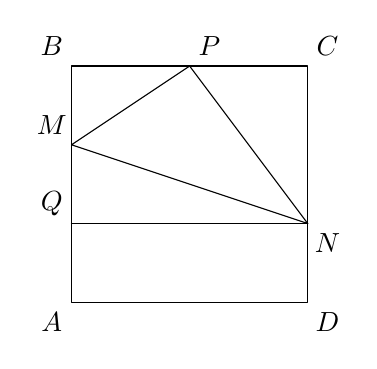
\begin{tikzpicture}[scale=1, line join=round, line cap=round]
			\coordinate (A) at (0,0); \coordinate (D) at (3,0); \coordinate (C) at (3,3);
			\coordinate (B) at (0,3);
			\coordinate (M) at (0,2);
			\coordinate (N) at (3,1);
			\coordinate (P) at (1.5,3);
			\coordinate (Q) at (0,1);
			\draw (A)--(D)--(C)--(B)--cycle; 
			\draw (P)--(M)--(N)--cycle;
			\draw (N)--(Q)--cycle;
			\draw (A)  node[shift={(-0.25,-0.25)}] {$A$};
			\draw (B)  node[shift={(-0.25,0.25)}] {$B$};
			\draw (D)  node[shift={(0.25,-0.25)}] {$D$};
			\draw (C)  node[shift={(0.25,0.25)}]  {$C$};
			\draw (M)  node[shift={(-0.25,0.25)}] {$M$};
			\draw (N)  node[shift={(0.25,-0.25)}] {$N$};
			\draw (P)  node[shift={(0.25,0.25)}] {$P$};
			\draw (Q)  node[shift={(-0.25,0.25)}] {$Q$};
		\end{tikzpicture}
		}
		}
\end{ex}

%%%Câu 4
\begin{ex}%[0D4-Bai2-Dang1-KQ]%[Dự án đề cương 3 Khối NH24-25-Dot 2- Bùi Lương Phúc]%[0H4H2-4]
Tam giác $ABC$ có $b(b^2 - a^2) = c(a^2 - c^2)$. Khi đó góc $A$ có số đo bằng bao nhiêu độ?
\par
\shortans{$60^\circ$}
\loigiai{
Ta có
\begin{align*}
b(b^2 - a^2)
= c(a^2 - c^2) \Leftrightarrow& b^3 + c^3 - a^2b - a^2c = 0 \\
\Leftrightarrow& (b + c)(b^2 - bc + c^2) - a^2(b + c) = 0\\
\Leftrightarrow& b^2 - bc + c^2 - a^2= 0\\
\Leftrightarrow& b^2 - a^2 + c^2 = bc\\
\Leftrightarrow& \dfrac{b^2 + c^2 - a^2}{2bc} = \dfrac{1}{2}\\
\Leftrightarrow& \cos A = \dfrac{1}{2}\\
\Leftrightarrow& A = 60^\circ.
\end{align*}
}
\end{ex}

%%%Câu 5
\begin{ex}%[0D4-Bai2-Dang2-KQ]%[Dự án đề cương 3 Khối NH24-25-Dot 2- Bùi Lương Phúc]%[0H4V2-2]
	(\textit{\footnotesize Trích đề thi CKI - THPT Nguyễn Thái Bình - TPHCM - Năm học 2024-2025})
	\immini{Gia đình bác An có mảnh đất như hình vẽ bên. Nhà nước có dự án xây bệnh viện nên thu hồi mảnh đất của bác, giá đền bù là $1{,}2$ triệu đồng trên mỗi mét vuông. Hỏi số tiền gia đình nhà bác An nhận được khoảng bao nhiêu triệu đồng (làm tròn kết quả đến hàng đơn vị)?
	}{
		\begin{tikzpicture}[scale=1, font=\footnotesize, line join=round, line cap=round,>=stealth]
			\coordinate (A) at (0,0);
			\coordinate (B) at ($(A)-(-1.5,3.5)$);
			\coordinate (C) at ($(B)+(2.9,0)$);
			\coordinate (D) at ($(C)+(1.8,4.5)$);
			\draw (A) -- (B) -- (C) -- (D) -- cycle;
			\draw (A) -- (D) node[midway, above] {$22$\,m};
			\draw (A) -- (B) node[midway, left] {$15$\,m};
			\draw (C) -- (D) node[midway, right] {$18$\,m};
			\draw (B) -- (C) node[midway, below] {$10$\,m};
			\draw pic["$73{,}07^\circ$", draw=black, angle radius=0.4cm, angle eccentricity=2] {angle=B--A--D};
			\foreach \p/\pos in {A/left, B/below, C/below, D/right}
			\node[\pos] at (\p) {{$\p$}};
		\end{tikzpicture}
	}
	\par
	\shortans{$294$}
	\loigiai{
		Diện tích tam giác $ABD$ bằng $S_{\triangle ABD}=\dfrac{1}{2}\cdot 22 \cdot 15 \cdot \sin 73{,}07^\circ \approx 157{,}85$.\\
		Áp dụng định lí côsin ta có\\
		$BD = \sqrt{15^2 + 22^2 - 2 \cdot 15 \cdot 22 \cdot \cos73{,}07^\circ}\approx 22{,}73$.\\
		$p = \dfrac{BC + CD + BD}{2} = \dfrac{10 + 18 + 22{,}73}{2}$.\\
		Diện tích tam giác $BCD$ bằng $S_{\triangle BCD} = \sqrt{p(p - BC)(p - CD)(p - BD)}
		\approx 86{,}97$.\\
		Từ đó số tiền mà gia đình bác An nhận được là $\left( 157{,}84+86{,}97\right)  \cdot 1{,}2 \approx 294$ (triệu đồng).}
\end{ex}
\Closesolutionfile{ans}


\ind{PHẦN IV.} \inden{Tự luận.}\\
\setcounter{ex}{0}

%%%===Câu 1==
\begin{ex}%[0D4-Bai2-Dang1-TL]%[Dự án đề cương 3 Khối NH24-25-Dot 2- Bùi Lương Phúc]%[0H4H2-1]
Tam giác $ABC$ có $a=6$, $b=4\sqrt{2}$, $c=2$. Gọi $M$ là điểm trên cạnh $BC$ sao cho $BM=3$. Tính độ dài đoạn $AM$.
\dapso{$3$}
\loigiai
{
\begin{center}
\begin{tikzpicture}[scale=1, font=\footnotesize, line join=round, line cap=round, >=stealth]
\coordinate[label = left:$B$] (B) at (0,0);
\coordinate[label = right:$C$] (C) at ($(B)+(6,0)$);
\coordinate[label = above:$A$, shift=(70.53:2cm)] (A) at (B);
\coordinate[label = below:$M$] (M) at ($(B)!0.5!(C)$);
\coordinate[label = left:$2$] (I) at ($(A)!0.5!(B)$);
\coordinate[label = below:$3$] (J) at ($(B)!0.5!(M)$);
\coordinate[label = above:$4\sqrt{2}$] (K) at ($(A)!0.5!(C)$);
\draw (C)--(B)--(A)--cycle (A)--(M);
\foreach \x in {A,B,C,M} \fill (\x) circle (1pt);
\end{tikzpicture}
\end{center}
Trong tam giác $ABC$, ta có
\[
\cos B = \dfrac{a^2 + c^2 - b^2}{2ac}
= \dfrac{6^2 + 2^2-\left(4\sqrt{2}\right)^2}{2 \cdot 6\cdot2}
= \dfrac{1}{3}.
\]
Trong tam giác $ABM$, ta có
\[
AM^2= AB^2+BM^2-2AB\cdot BM\cdot\cos B = 4+9-2\cdot 2\cdot 3\cdot\dfrac{1}{3}
= 9\Rightarrow AM =3.
\]
\ding{43}Cách khác:
Dễ thấy tam giác $ABC$ vuông tại $A$ và $M$ là trung điểm của $BC$ nên \[AM=\dfrac{1}{2}BC=\dfrac{1}{2}\cdot 6= 3.\]
}
\end{ex}

%%%==Câu 2==
\begin{ex}%[0D4-Bai2-Dang1-TL]%[Dự án đề cương 3 Khối NH24-25-Dot 2- Bùi Lương Phúc]%[0H4H2-1]
Cho tam giác $ABC$ có $AB=3,\ BC=5$ và độ dài đường trung tuyến $BM=\sqrt{13}$. Tính độ dài $AC$.
\par
\dapso{$4$}
\loigiai{
\begin{center}
\begin{tikzpicture}[scale=1, font=\footnotesize, line join=round, line cap=round, >=stealth]
\coordinate[label = left:$B$] (B) at (0,0);
\coordinate[label = right:$C$] (C) at ($(B)+(5,0)$);
\coordinate[label = above:$A$, shift=(53.13:3cm)] (A) at (B);
\coordinate[label = above right:$M$] (M) at ($(A)!0.5!(C)$);
\coordinate[label = left:$3$] (I) at ($(A)!0.5!(B)$);
\coordinate[label = below:$5$] (J) at ($(B)!0.5!(C)$);
\coordinate[label = above:$\sqrt{13}$] (J) at ($(B)!0.5!(M)$);
\draw (C)--(B)--(A)--cycle (B)--(M);
\foreach \x in {A,B,C,M} \fill (\x) circle (1pt);
\end{tikzpicture}
\end{center}
Đặt $AC=b$.	Trong tam giác $ABC$, ta có
\[
\cos A = \dfrac{b^2 + c^2 - a^2}{2bc}
= \dfrac{b^2 + 3^2-5^2}{2 \cdot b\cdot3}
= \dfrac{b^2 -16}{6b}\qquad(1).
\]
Trong tam giác $ABM$, ta có
\[
\cos A = \dfrac{AB^2 + AM^2 - BM^2}{2AB\cdot AM}
= \dfrac{3^2 + \dfrac{b^2}{4}-\left(\sqrt{13}\right)^2}{2 \cdot 3\cdot \dfrac{b}{2}}
= \dfrac{\dfrac{b^2}{4}-4}{3b}\qquad(2).
\]
Từ ($1$) và ($2$) suy ra, \\
\[\dfrac{b^2 -16}{6b}=\dfrac{\dfrac{b^2}{4}-4}{3b}\Leftrightarrow b^2 -16=0\Leftrightarrow b=4.\]
Vậy $AC=4$.\\
\begin{khung4}{Chú ý}
	\ding{43} \textbf{Chú ý:}
Trong tam giác $ABC$, đường trung tuyến $BM$ có thể tính như sau:
\[
\cos A = \dfrac{b^2 + c^2 - a^2}{2bc}\qquad(a).
\]
Trong tam giác $ABM$, ta có
\[
\cos A = \dfrac{AB^2 + AM^2 - BM^2}{2AB\cdot AM}\qquad(b).
\]
Từ ($a$) và ($b$) suy ra, \\
\[\dfrac{b^2 + c^2 - a^2}{2bc}=\dfrac{c^2 + \left(\dfrac{b}{2}\right)^2 - BM^2}{2c\cdot \dfrac{b}{2}}.\]
Tiếp tục tính $BM$ ta thu được $BM^2 = \dfrac{c^2 + a^2}{2} - \dfrac{b^2}{4}$.\\
Hay
\[\boxed{m_b = \sqrt{\dfrac{c^2 + a^2}{2} - \dfrac{b^2}{4}}}
\]
\end{khung4}
}
\end{ex}

%%%==Câu 3==
\begin{ex}%[0D4-Bai2-Dang1-TN]%[Dự án đề cương 3 Khối NH24-25-Dot 2- Bùi Lương Phúc]%[0H4H2-4]
	Cho tam giác $ABC$ có $BC=a$, $AC=b$, $AB=c$, có $a^2 = b^2 + c^2 + bc\sqrt{2}$. Tính số đo của góc $A$.
	\par
	\dapso{$135^\circ$}
	\loigiai
	{
		Ta có $\cos A = \dfrac{b^2 + c^2 - a^2}{2bc} = \dfrac{-bc\sqrt{2}}{2bc} = -\dfrac{\sqrt{2}}{2} \Rightarrow \widehat{A} = 135^\circ$.
	}
\end{ex}

%%%==Câu 4==
\begin{ex}%[0D4-Bai2-Dang1-TN]%[Dự án đề cương 3 Khối NH24-25-Dot 2- Bùi Lương Phúc]%[0H4H2-4]
	(\textit{\footnotesize Trích đề thi GKI - THPT Chuyên Trần Phú - Hải Phòng - Năm học 2024-2025})\\
Cho tam giác $ABC$ có góc $C$ nhọn và $AC=3$, $BC=4$, $S_{ABC}=3\sqrt{3}$. Tính độ dài cạnh $AB$.
\par
\dapso{$3{,}6$}
\loigiai{
\[
S=\dfrac{1}{2}AC\cdot BC\sin C=\dfrac{1}{2}\cdot3\cdot4\sin C=6\sin C.
\]
Do $S=3\sqrt{3}$, suy ra
\[
6\sin C=3\sqrt{3}\Rightarrow \sin C=\dfrac{\sqrt{3}}{2}.
\]
Vì góc $\widehat C$ là góc nhọn nên $C=60^\circ$.\\
Áp dụng định lý côsin
\[
AB^2=AC^2+BC^2-2\cdot AC\cdot BC\cos C
=3^2+4^2-2\cdot3\cdot4\cos60^\circ=9+16-2\cdot3\cdot4\cdot\dfrac{1}{2}=25-12=13.
\]
Do đó $AB=\sqrt{13}$.
}
\end{ex}
%%%==Câu 5==
\begin{ex}%[0D4-Bai2-Dang1-TL]%[Dự án đề cương 3 Khối NH24-25-Dot 2- Bùi Lương Phúc]%[0H4H2-2]
	(\textit{\footnotesize Trích đề thi CKI - THPT Chuyên Trần Phú - Hải Phòng - Năm học 2024-2025})\\
	Cho tam giác $ABC$, biết các cạnh $a=3$, $b=4$, $c=6$. Tính độ đài đường cao hạ từ đỉnh $C$ của tam giác (làm tròn kết quả đến hàng phần trăm).
	\dapso{$1{,}78$}
	\loigiai{
		\immini{
			Ta gọi $h_c$ là đường cao ứng với đỉnh $C$.\\
			Theo công thức diện tích, ta có\\
			$S=\sqrt{p(p-a)(p-b)(p-c)}$ với $p=\dfrac{a+b+c}{2}=\dfrac{13}{2}$.\\
			Nên $S=\sqrt{\dfrac{13}{2}\left(\dfrac{13}{2}-3\right)\left(\dfrac{13}{2}-4\right)\left(\dfrac{13}{2}-6\right)}=\dfrac{\sqrt{455}}{4}$.\\
			Ta có $h_c=\dfrac{2 S}{c}=\dfrac{\sqrt{455}}{2\cdot 6}=\dfrac{\sqrt{455}}{12} \approx 1{,}78$.}{
			\begin{tikzpicture}[scale=1, font=\footnotesize, line join=round, line cap=round, >=stealth]
				\coordinate[label = left:$B$] (B) at (0,0);
				\coordinate[label = right:$A$] (A) at ($(B)+(6,0)$);
				\coordinate[label = above:$C$, shift=(26.4:4cm)] (C) at (B);
				\coordinate[label = below:$H$] (H) at ($(B)!(C)!(A)$);
				\draw (A)--(B)--(C)--cycle (C)--(H);
				\foreach \x in {A,B,C,H} \fill (\x) circle (1pt);
				\newcommand{\gocv}[4][black]{\draw[#1] ($(#3)!5pt!(#2)$)--($(#3)!2!($($(#3)!5pt!(#2)$)!.5!($(#3)!5pt!(#4)$)$)$)--($(#3)!5pt!(#4)$);} 
				\gocv{A}{H}{C};
			\end{tikzpicture}
		}
	}
\end{ex}
%%%==Câu 6==
\begin{ex}%[0D4-Bai2-Dang1-TL]%[Dự án đề cương 3 Khối NH24-25-Dot 2- Bùi Lương Phúc]%[0H4V2-3]
	(\textit{\footnotesize Trích đề thi GKI - THPT Phạm Phú Thứ - Tp HCM - Năm học 2024-2025})\\
	Gọi $h_a$, $h_b$, $h_c$ lần lượt là độ dài đường cao xuất phát từ đỉnh $A$, $B$, $C$ của tam giác $ABC$ và $r$ là bán kính đường tròn nội tiếp tam giác $ABC$. Chứng minh rằng
	\[\dfrac{1}{r} = \dfrac{1}{h_a} + \dfrac{1}{h_b} + \dfrac{1}{h_c}.
	\]
	\dapso{}
	\loigiai{
		Ta có
		\begin{itemize}
			\item $S = \dfrac{1}{2}h_a\cdot a \Rightarrow \dfrac{1}{h_a} = \dfrac{a}{2S}$.
			\item $S = \dfrac{1}{2}h_b\cdot b \Rightarrow \dfrac{1}{h_b} = \dfrac{b}{2S}$.
			\item $S = \dfrac{1}{2}h_c\cdot c \Rightarrow \dfrac{1}{h_c} = \dfrac{c}{2S}$.
			\item $S = pr$ với $p = \dfrac{a + b + c}{2}$.
		\end{itemize}
		Do đó
		\begin{eqnarray*}
			\dfrac{1}{h_a} + \dfrac{1}{h_b} + \dfrac{1}{h_c} = \dfrac{a}{2S} + \dfrac{b}{2S} + \dfrac{c}{2S} = \dfrac{a + b + c}{2S} = \dfrac{a + b + c}{2}\cdot \dfrac{1}{S} = p\cdot \dfrac{1}{pr} = \dfrac{1}{r}.
		\end{eqnarray*}
		Vậy $\dfrac{1}{r} = \dfrac{1}{h_a} + \dfrac{1}{h_b} + \dfrac{1}{h_c}$.
	}
\end{ex}
%%%==Câu 7==
\begin{ex}%[0D4-Bai2-Dang1-TL]%[Dự án đề cương 3 Khối NH24-25-Dot 2- Bùi Lương Phúc]%[0H4V2-1]
	Cho hình bình hành $ABCD$ có $AB = 3$, $BC = 2\sqrt{2}$, góc $B$ tù và diện tích hình bình hành bằng $6$. Tính độ dài đường chéo $BD$ (kết quả làm tròn đến hàng phần trăm).
	\dapso{$2{,}24$}
	\loigiai{
		\begin{center}
			\begin{tikzpicture}[scale=0.8, font=\footnotesize, line join=round, line cap=round, >=stealth]
				\def\d{4}
				\def\r{3}
				\path (0:0) coordinate (A)
				++(0:\d) coordinate (B)
				++(50:\r) coordinate (C)
				($(A)+(C)-(B)$) coordinate (D);
				\draw (A)--(B)--(C)--(D)--cycle (B)--(D);
				\foreach \x/ \goc in {A/180,B/0,C/0,D/180} 
				\fill (\x) circle (1pt)	
				($(\x)+(\goc:3mm)$) node {$\x$};
			\end{tikzpicture}
		\end{center}
		Ta có $S_{\triangle ABC}=\dfrac{1}{2}\cdot S_{ABCD}=3$\hfill (1)\\
		Mà $S_{\triangle ABC}=\dfrac{1}{2}\cdot BA\cdot BC\cdot \sin B=\dfrac{1}{2}\cdot 3\cdot 2\sqrt{2}\cdot \sin B=3\sqrt{2}\sin B$\hfill (2)\\
		Từ (1) và (2) suy ra $\sin B=\dfrac{1}{\sqrt{2}}$. Do $\widehat{B}$ tù nên $\widehat{B}=135^\circ\Rightarrow \widehat{DAB}=45^\circ$.\\
		Áp dụng định lí côsin trong tam giác $ABD$ có
		\begin{eqnarray*} 
			BD&=&\sqrt{AB^2+AD^2-2\cdot AB\cdot AD\cdot \cos\widehat{DAB}}\\
			&=&\sqrt{9^2+(2\sqrt{2})^2-2\cdot 3\cdot 2\sqrt{2}\cdot\cos 45^\circ}=\sqrt{5}\approx 2{,}24.
		\end{eqnarray*}
	}
\end{ex}
%%%==Câu 8==
	\begin{ex}%[0D4-Bai2-Dang2-TL]%[Dự án đề cương 3 Khối NH24-25-Dot 2- Bùi Lương Phúc]%[0H4V3-2]
		\immini{Để kéo dây điện từ cột điện vào nhà phải qua một cái ao, anh Nam không thể đo độ dài dây điện cần mua trực tiếp được nên đã làm như sau: Lấy một điểm $B$ như trong hình, người ta đo được độ dài từ $B$ đến $A$ (nhà) là $15$\,m, từ $B$ đến $C$ (cột điện) là $18$\,m và $\widehat{ABC}=120^\circ$. Tính độ dài dây điện nối từ nhà ra đến cột điện (làm tròn kết quả đến hàng phần chục).}{
			\begin{tikzpicture}[>=stealth,line join=round,line cap=round,font=\footnotesize,scale=1]
				\def\m{4.1} \def\n{2.7} \def\p{2.5}
				\path
				(0,0) coordinate (A)
				(\p,0) coordinate (B)
				(\m,\n) coordinate (C);
				\foreach \ptA/\ptC/\pos in {C/A/above, A/B/below, B/C/below} {
					\draw(\ptA) -- (\ptC);
					\fill(\ptA) circle (1pt);
					\node[\pos] at (\ptA) {$\ptA$};
				}
				\fill(B) circle (1pt);
				\node[below] at (B) {$B$};
				\path let \p1 = (A), \p2 = (B) in
				node[below] at ($(\p1)!.5!(\p2)$) {$15$\,cm};
				\path let \p2 = (B), \p3 = (C) in
				node[below,rotate=60] at ($(\p2)!.5!(\p3)$) {$18$\,cm};
				\draw pic[draw,angle radius=2.5mm,angle eccentricity=2,"$\scriptsize 120^\circ$"] {angle = C--B--A}; 
				\begin{scope}[gray, thick, fill=green!40!gray,scale=0.6,xshift=-0.3cm,yshift=1.4cm,opacity=0.9]
					\coordinate (E) at (0,0);
					\coordinate (F) at (6,2);
					\coordinate (Control1a) at (-0.5,1.1);
					\coordinate (Control1b) at (5.7,3);
					\coordinate (Control2a) at (6.4,0);
					\coordinate (Control2b) at (1,-1.8);			
					\draw[gray, thick, fill=gray!50]
					(E) .. controls (Control1a) and (Control1b) .. (F)
					.. controls (Control2a) and (Control2b) .. cycle;	
				\end{scope}
			\end{tikzpicture}
		}
		\dapso{$28{,}6$}
		\loigiai{
			Áp dụng định lí côsin cho tam giác $ABC$ ta có\\
			\[AC=\sqrt{AB^2+BC^2-2AB\cdot BC\cdot \cos B}=\sqrt{15^2}+18^2-2\cdot 15\cdot 18\cdot \cos 120^\circ\approx 28{,}62\ \text{(m)}.\]
			Vậy độ dài dây điện nối từ nhà ra cột điện dài $28{,}6$\,m.
		}
	\end{ex}
%%%%==Câu 9==
\begin{ex}%[0D4-Bai2-Dang2-TL]%[Dự án đề cương 3 Khối NH24-25-Dot 2- Bùi Lương Phúc]%[0H4V3-2]
\immini{
Tàu $A$ cách cảng $C$ một khoảng $3$\,km và lệch hướng bắc một góc $47{,}45^\circ$. Tàu $B$ cách cảng $C$ một khoảng $5$\,km và lệch hướng bắc một góc $112{,}90^\circ$ (Hình vẽ bên). Hỏi khoảng cách giữa hai tàu là bao nhiêu ki-lô-mét (làm tròn kết quả đến hàng phần trăm)?
}{
\begin{tikzpicture}[scale=1, font=\footnotesize, line join=round, line cap=round, >=stealth]
\coordinate[label = left:$C$] (C) at (0,0);
\coordinate[label = right:$N$] (N) at ($(C)+(0,3.5)$);
\coordinate[label = above:$A$, shift=(42.15:3cm)] (A) at (C);
\coordinate[label = right:$B$, shift=(-22.9:5cm)] (B) at (C);
\draw (A)--(C)--(B);
\draw[->] (C)--(N);
\draw[dashed] (A)--(B);
\foreach \x in {A,B,C,N} \fill (\x) circle (1pt);
\draw pic["$47{,}45^\circ$"{xshift=3pt}, draw=black, angle radius=0.5cm, angle eccentricity=1.4,double] {angle=A--C--N};
\draw pic["$112{,}9^\circ$"{yshift=-9pt}, draw=black, angle radius=1.1cm, angle eccentricity=1.5] {angle=B--C--N};
\end{tikzpicture}
}
\dapso{$4{,}64$}
\loigiai{
Ta có: $\widehat{ACB} = 112{,}90^\circ - 47{,}45^\circ = 65{,}45^\circ$.\\
Áp dụng định lý cô-sin cho tam giác $ABC$, ta được:
\begin{align*}
AB^2 &= AC^2 + BC^2 - 2\cdot AC \cdot BC \cdot \cos \widehat{ACB} \\
&= 3^2 + 5^2 - 2\cdot 3 \cdot 5 \cdot \cos 65{,}45^\circ \\
&\approx 21{,}54.
\end{align*}
Suy ra $AB \approx \sqrt{21{,}54} \approx 4{,}64$\,km.\\
Vậy khoảng cách giữa hai tàu là khoảng $4{,}64$\,km.
}
\end{ex}

%%%%==Câu 10==
\begin{ex}%[0D4-Bai2-Dang2-TL]%[Dự án đề cương 3 Khối NH24-25-Dot 2- Bùi Lương Phúc]%[0H4V3-2]
\immini{
Từ một phần của miếng tôn hình tròn, người ta cắt ra được một tam giác $ABC$ có $AB = 6$ cm, $AC = 8$ cm, $\widehat{A} = 150^\circ$ (Hình vẽ bên).
Hãy tính:
\begin{itemize}
\item[a)] Bán kính của miếng tôn ban đầu (làm tròn đến hàng phần mười, đơn vị cm).
\item[b)] Diện tích tam giác $ABC$.
\end{itemize}}{
\begin{tikzpicture}[scale=1, font=\footnotesize, line join=round, line cap=round, >=stealth]
\def\r{4}
\coordinate (I) at (0,0);
\coordinate (E) at (\r,0);
\coordinate (F) at ({\r*cos(120)},{\r*sin(120)});
\coordinate (H) at ($(\r,0)+(-3,0.7)$);
\fill[pattern=north east lines, shading=axis, left color=red!20, right color=yellow!40, opacity=0.7]
(E)
-- ($(E)+(-0.7,0.3)$)
.. controls +(-0.8,0) .. (H)
.. controls +(-0.9,1.4) .. ($(F)+(0.3,-0.5)$)
-- (F)
arc[start angle=120, end angle=0, radius=\r]
-- cycle;
\draw[blue, thick] (E) arc[start angle=0, end angle=120, radius=\r];
\pgfmathsetmacro{\v}{0.78}
\pgfmathsetmacro{\u}{0.57}
\pgfmathsetmacro{\t}{0.26}
\pgfmathsetmacro{\angleE}{0}
\pgfmathsetmacro{\angleF}{120}
\pgfmathsetmacro{\angleA}{\angleE + (\angleF - \angleE)*\v}
\coordinate (A) at ({\r*cos(\angleA)},{\r*sin(\angleA)});
\pgfmathsetmacro{\angleB}{\angleE + (\angleF - \angleE)*\u}
\coordinate (B) at ({\r*cos(\angleB)},{\r*sin(\angleB)});
\pgfmathsetmacro{\angleC}{\angleE + (\angleF - \angleE)*\t}
\coordinate (C) at ({\r*cos(\angleC)},{\r*sin(\angleC)});
%		\fill (I) circle (1pt) node[below] {$I$};
\fill (E) circle (1pt) node[right] {$E$};
\fill (F) circle (1pt) node[above] {$F$};
\fill (A) circle (1pt) node[above ] {$A$};
\fill (B) circle (1pt) node[above ] {$B$};
\fill (C) circle (1pt) node[above right] {$C$};
\draw[red, thick] (E)--($(E)+(-0.7,0.3)$) .. controls +(-0.8,0) .. (H);
\draw[red, thick] (H) .. controls +(-0.9,1.4) .. ($(F)+(0.3,-0.5)$)-- (F);
\draw(C) -- (A)--(B)--cycle;
%		\draw pic[fill=gray,angle radius=2.5mm,angle eccentricity=1.6] {angle = A--C--B};
\draw pic[draw,angle radius=2.5mm,angle eccentricity=1.9,"$\scriptsize 150^\circ$",pic text options={xshift=9pt}] {angle = A--B--C}; 
%\tkzMarkAngle[size=.04*\r](A,B,C)
%\tkzLabelAngle[pos=0.35,xshift=4pt](A,B,C){\scriptsize $150^\circ$}
\end{tikzpicture}
}
\dapso{$13{,}5$\ \text{và}\ $12$}
\loigiai{
Áp dụng định lý cô-sin trong tam giác $ABC$, ta có
\begin{align*}
BC^2 &= AB^2 + AC^2 - 2\cdot AB \cdot AC \cdot \cos \widehat{A} \\
&= 6^2 + 8^2 - 2 \cdot 6 \cdot 8 \cdot \cos 150^\circ \\
&\approx 36 + 64 + 83{,}14 = 183{,}14.
\end{align*}
Suy ra $BC \approx \sqrt{183{,}14} \approx 13{,}5$\,cm.\\
a) Áp dụng định lý sin $\dfrac{BC}{\sin A} = 2R \Rightarrow R = \dfrac{BC}{2\sin A} \approx \dfrac{13{,}5}{2 \cdot \sin 150^\circ} = 13{,}5$\,cm.\\
b) Diện tích tam giác
\[
S = \dfrac{1}{2} \cdot AB \cdot AC \cdot \sin A = \dfrac{1}{2} \cdot 6 \cdot 8 \cdot \sin 150^\circ = 12\ \text{cm}^2.
\]
}
\end{ex}

















































